\documentclass[a4paper,12pt,twoside]{book}\usepackage[utf8]{inputenc}
\usepackage[english]{babel}
\usepackage{hyperref}
\usepackage{siunitx}
\usepackage{graphicx}
\usepackage{biblatex}
\usepackage{physics}
\usepackage{amsmath}

\usepackage{xcolor}
\usepackage{listings}
\usepackage{minted}
\paperheight=297mm
\paperwidth=210mm

\setlength{\textheight}{235mm}
\setlength{\topmargin}{-1.2cm} % pour centrer la page verticalement
%\setlength{\footskip}{5mm}
\setlength{\textwidth}{15cm}
\setlength{\oddsidemargin}{0.56cm}
\setlength{\evensidemargin}{0.56cm}

\pagestyle{plain}

\usepackage[top=1.5cm, bottom=1.5cm, left=2.0cm, right=2.0cm]{geometry}

\addbibresource{sample.bib}

\title{Quantum Technology project on Superconducting Circuits}
\author{Francesco Adinolfi, Moritz Fontboté Schmidt, Yongxin Song, \\ Alperen Tugen}
\date{June 2020}


%% My own little command library

\providecommand{\e}[1]{\ensuremath{\cdot10^{#1}}}
\providecommand{\half}{\ensuremath{\frac{1}{2}}} %unedemie
\providecommand{\const}{\ensuremath{\text{const}}} %const en lettres
\providecommand{\eval}[1]{\ensuremath{\Big|_{#1}}} % evalue
\providecommand{\ehat}{\ensuremath{\hat{\pmb e}}} %ê 
\providecommand{\degre}{\ensuremath{{^\circ}}} % ° 
\def\restrict#1{\raise-.5ex\hbox{\ensuremath|}_{#1}} % restreindre une fonction
\def\doubleunderline#1{\underline{\underline{#1}}}

% Partielles
\providecommand{\dtheta}[1]{\ensuremath{\frac{\partial #1}{\partial \theta}}}
\providecommand{\dt}[1]{\ensuremath{\frac{\partial #1}{\partial t}}}
\providecommand{\dz}[1]{\ensuremath{\frac{\partial #1}{\partial z}}}
\providecommand{\dx}[1]{\ensuremath{\frac{\partial #1}{\partial x}}}
\providecommand{\dxx}[1]{\ensuremath{\frac{\partial^2 #1}{\partial x^2}}}
\providecommand{\dr}[1]{\ensuremath{\frac{\partial #1}{\partial r}}}
\providecommand{\Div}[0]{\ensuremath{\nabla \cdot}} % divergence
\providecommand{\Grad}[0]{\ensuremath{\nabla}} % gradient
\providecommand{\Rot}[0]{\ensuremath{\nabla \wedge}} % gradient
\providecommand{\Lapl}[0]{\ensuremath{\nabla^2}} % laplacien
\providecommand{\p}[0]{\partial} % partiel



%evalue

% parentheses, matrices et tt ça
\providecommand{\lrp}[1]{\ensuremath{\left(#1\right)}}
\providecommand{\bmat}[1]{\begin{bmatrix}#1\end{bmatrix}} %bracketmatrix
% \newcommand{\norm}[1]{\left\lVert#1\right\rVert} % norm
\providecommand{\abs}[1]{\lvert #1 \rvert} %abs


\providecommand{\eqdef}[0]{\mathrel{\overset{\makebox[0pt]{\mbox{\normalfont\tiny\sffamily def}}}{=}}} % =def 
\providecommand{\eqwrite}[1]{\mathrel{\overset{\makebox[0pt]{\mbox{\normalfont\tiny\sffamily \ensuretext{#1}}}}{=}}} % ecrire au desssus d'equation 
\providecommand{\eqwritemath}[1]{\mathrel{\overset{\makebox[0pt]{\mbox{\normalfont\tiny\sffamily {#1}}}}{=}}} % ecrire au desssus d'equation 

\includeonly{chap_introduction} 

\begin{document}

\maketitle
\tableofcontents

\chapter{Introduction}


\chapter{Transmon qubit}

\section{The Josephson Junction}
The Josephson junction could be considered as one of the most elementary block of Superconducting Qubits. \\
It is composed by:
\begin{itemize}
    \itemsep0em 
    \item central thin layer of insulator ($Al_{2}O_{3}$),
    \item two external layers of superconducting material (Al, Nb)
\end{itemize}
A basic sketch of the the Josephson Junction is showed in Fig. \ref{fig:jj1}

\begin{figure}[h]
\centering
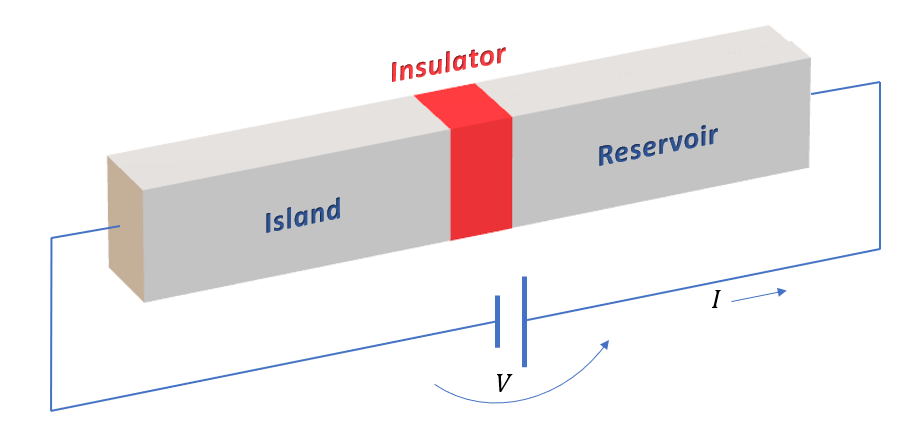
\includegraphics[width=0.7\textwidth]{pic/transmon/jj1.png}
\caption{Josephson Junction connected to a voltage source}
\label{fig:jj1}
\end{figure}

When the junction is cooled down below its critical temperature $Tc$ the behaviour of the component dramatically changes. By specific kind of interaction among couple of electrons with the lattice cooper pairs are formed. This effective particles, with bosonic character, can flow inside the superconductors without encountering any kind of resistance.\\
Let's suppose to write the two Ginzburg-Landau order parameter associated to the two superconducting regions:
\begin{equation}\begin{split}
\psi_{A} = \sqrt{n_{A}}\exp{i\phi_{A}}\\
\psi_{B} = \sqrt{n_{B}}\exp{i\phi_{B}}
\end{split}\end{equation}
which could be interpreted as the wave functions describing the behaviour of cooper-pairs. Considering a constant Voltage applied $V$ across the junction the energy difference for each cooper-pair will be $2eV$.
The Schroedinger equation for this system will be:
\begin{equation}
    \begin{split}
        i\hbar\frac{\partial \psi_{A}}{\partial t} = eV\psi_{A} + K\psi_{B}\\
        i\hbar\frac{\partial \psi_{B}}{\partial t} = eV\psi_{B} + K\psi_{A}
    \end{split}
\end{equation}

From this starting setting we could derive the final relations:
\begin{gather}
     I = \frac{dn_A}{dt} = \frac{2\sqrt{n_An_B}}{\hbar} Ksin(\delta)\\
    \frac{d\delta}{dt} = \frac{2eV}{\hbar} 
\end{gather}
 where $I$ is the current flowing inside the junction, $n_A, n_B$ the cooper-pair density associated to the superconducting junctions and $\delta$ is defined as the phase difference of the Ginzburg-Landau parameter along the junction:
 \begin{equation}
     \delta = \phi_{A} - \phi_{B} 
 \end{equation} 
 
 
 
\section{Cooper Pair Box}

\begin{figure}[h]
\centering
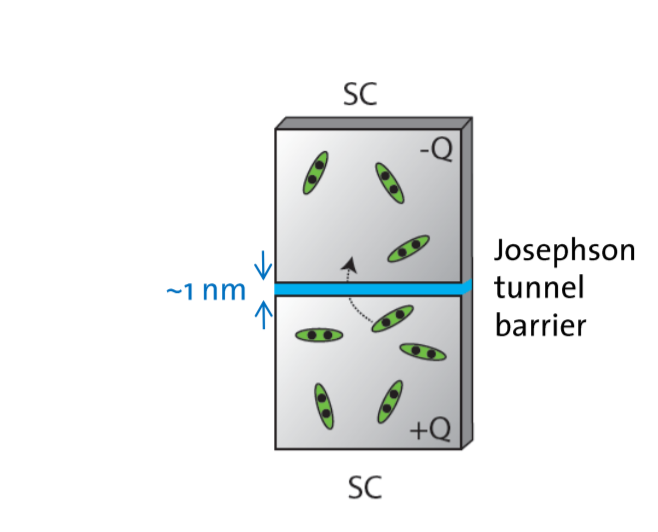
\includegraphics[width=0.4\textwidth]{pic/transmon/jj3.png}
\caption{Cooper pairs tunneling the Josephson junction}
\end{figure}
Starting from this macroscopic introduction, let's study how to write the main form of the Hamiltonian for a Josephson junction subject to a Voltage across it.
We could label the two superconducting areas of the Junction respectively 'Island' and 'Reservoir'. When we apply a constant Voltage electrons can be transferred from the reservoir to the island by tunneling through the thin layer of insulator.\\
We suppose that both the island and reservoir behaves as good BCS superconductors which requires the following condition to be respected $$\Delta << K_BT,\frac{e^2}{2C_{\Sigma}} $$ where $\Delta$ is the superconducting energy gap, $K_BT$ is the thermal fluctuations energy, $\frac{e^2}{2C_{\Sigma}}$ Coulomb energy of the island.\\ \par 
Under this condition we could suppose all electrons are paired and have become cooper-pairs.
We could now focus on the number of cooper-pairs contained inside the island in excess with respect to the reservoir \textbf{n} which is linked to the total charge though  $q = -2ne$ . \footnote{$n$ could assume integer values. If $n = 0$ then we would have charge neutrality across the junction.}\\ 
Since cooper pairs in the island could fluctuate by quantum tunneling between island and reservoir we will describe $n$ by its quantum operator $$n \rightarrow \hat{n}$$
with basis-eigenstates 
\begin{equation}
    \hat{n}\ket{n} = n\ket{n}
\end{equation}

Moreover to describe the condensate wave function of cooper-pairs  it will  be useful also to define the phase operator 
\begin{equation}
\delta \rightarrow \hat{\delta}
\end{equation} 

and an alternative state basis 

\begin{equation} 
\ket{\delta} =  \sum_{n= -\infty}^{\infty} e^{in\delta}\ket{n}
\end{equation}

Performing more detailed calculation (see Appendix) it is possible to obtain the following useful relations:
\begin{equation}
    \begin{split}\label{eq:delta}
        e^{i\hat{\delta}} = \sum_{n= -\infty}^{\infty} \ket{n}\bra{n+1}\\
        e^{-i\hat{\delta}} = \sum_{n= -\infty}^{\infty} \ket{n+1}\bra{n}\\
    \end{split}
\end{equation}
\begin{equation}
    \label{eq:delta1}
    \hat{n} = \frac{1}{i}\frac{\partial}{\partial\delta}
\end{equation}

\subsection{Tunneling Hamiltonian}
In order to model the tunneling behavior of cooper-pairs across the junction we could define the following effective Hamiltonian

\begin{equation}
    H_J = -\frac{E_J}{2}\sum_{n=-\infty}^{\infty} (\ket{n}\bra{n+1} +\ket{n+1}\bra{n})
\end{equation}

Using eq. \ref{eq:delta} it is possible to rewrite the Hamiltonian as

\begin{equation}
    H_J = -\frac{E_J}{2}(e^{i\hat{\delta}}+e^{-i\hat{\delta}}) = -\frac{E_J}{2}cos(\hat{\delta})
\end{equation}


\subsection{Electrostatic Hamiltonian}
Let's now have a look to the circuital sketch of the Josephson junction in fig. \ref{fig:jj2}. Considering the electrostatic energy of cooper-pairs we could write an Hamiltonian of the form:
\begin{figure}[h]
\centering
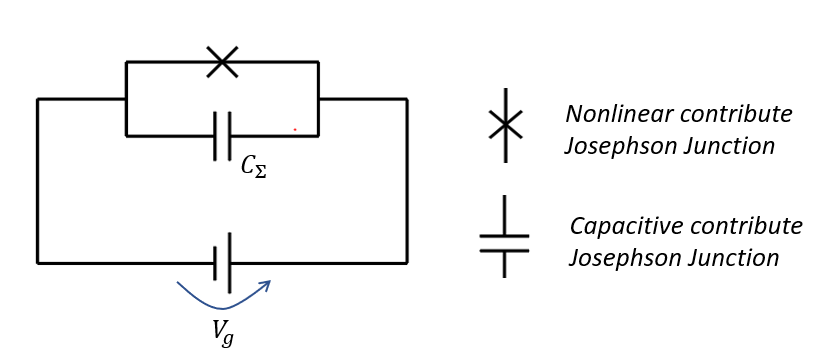
\includegraphics[width=0.7\textwidth]{pic/transmon/jj2.png}
\caption{Josephson Junction circuital sketch}
\label{fig:jj2}
\end{figure}



$$H_{el} = \frac{(2e)^2}{2C_{\Sigma}}\hat{n}^2 + 2e\hat{n}V_g  = 4E_C(\hat{n}-n_g)^2$$
   
with $E_C = \frac{e^2}{2C_{\Sigma}}$ and $n_g = \frac{C_{\Sigma}V_g}{2e}$ the number of cooper-pairs induced charge by the constant voltage $V_g$, and $C_{\Sigma}$ the total capacitance associated to the junction.\\
Actually what could happen, in general, is that we are never able to control exactly the value of $V_g$, due either to the presence of uncontrollable charge fluctuactions or noise. We describe in general $n_g$ as
\begin{equation}
    n_g = \frac{Q_r^2}{2e} + \frac{C_{\Sigma}V_g}{2e}
\end{equation}
where $Q_r$ represents the environment-induced offset charge.


\section{Solving the complete Hamiltonian}
Now let's compose all the parts to obtain the final Hamiltonian of the Cooper-pair box in phase representation
\begin{equation}
    \label{HamiltonianJJ}
    \begin{split}
    H = 4E_C(\hat{n}-n_g)^2 -E_Jcos(\hat{\delta}) \\= 4E_C(\frac{1}{i}\frac{\partial}{\partial\delta}-n_g)^2 -E_Jcos(\hat{\delta})
    \end{split}
\end{equation}
where we obtained the last equality using eq. \ref{eq:delta1} .\\
This would lead to the following Schrodinger equation
\begin{equation}
    4E_C(\frac{1}{i}\frac{\partial}{\partial\delta}-n_g)^2 -E_Jcos(\hat{\delta})\Psi(\delta) = E\Psi(\delta)
\end{equation}

As showed in more details in Appendix it is possible to solve this equation Mathieu functions obtaining the following result
\begin{equation}
    \Psi(\delta) = e^{in_g\delta}g(\frac{\delta}{2})\\
\end{equation}
where $g(\delta)$ could be obtained by solving the following differential equation
\begin{equation}
    g^{\prime\prime}(x) + [\frac{E}{E_C} + \frac{E_J}{E_C}cos(2x)]g(x) = 0
\end{equation}

We could also calculate the eigenergies (details in Appendix) which will  be given by
\begin{equation}
    E_m(n_g) = E_Ca_{[2n_g+k(m,n_g)]}(-\frac{E_J}{2E_C})
\end{equation}
with $a_x(y)$ Mathieu's characteristic value and $k(m,n_g)$ a function properly sorting the eigenvalues.\\
Plots the first eigenenergies $E_0(n_g), E_1(n_g),E_2(n_g)$ for different values of the ratio $E_J/E_C$ are shown in fig. \ref{fig:transmon}. 
\begin{figure}[h]
\centering
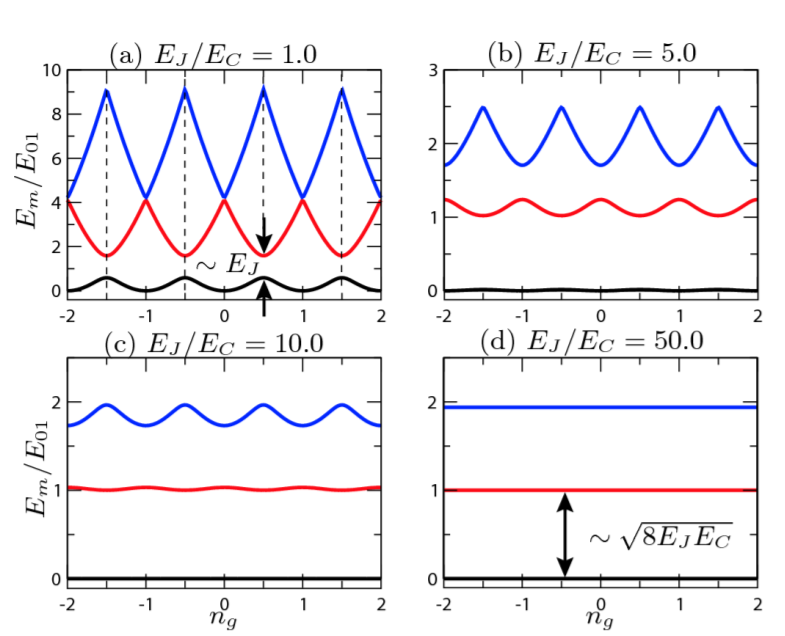
\includegraphics[width=0.7\textwidth]{pic/transmon/jj4.png}
\caption{Eigenenergies $E_0, E_1,E_2$ as a function of the offset charge  $n_g$ with different ratios of $E_J/E_C$. Energies are normalized with respect to $E_{01}$. Picture from \href{https://doi.org/10.1103/PhysRevA.76.042319}{Koch et al. PRA 2007}}
\label{fig:transmon}
\end{figure}

It is worth noticing that
\begin{itemize}
    \item the anharmonicity of the junction depends on the ratio $E_J/E_C$
    \item the eigenenergies fluctuations wrt to $n_g$ decrease very rapidly as $E_J/E_C$ increases
\end{itemize}
Having a high anharmonicity would help us in addressing selectively the $\ket{0} \longleftrightarrow \ket{1}$ while having small eigenergies fluctuations would stabilize the energy levels with respect to some external noise changing $n_g$


\section{Transmon regime}
The sensitivity of the qubit with respect to the charge offset fluctuations $n_g$ is important for increasing the coherence time $T_2$ of the qubit as mushc as possible. In view of this working in the transmon regime is of vital importance. The transmon regime is defined when the condition $$\frac{E_J}{E_C} >> 1$$  is met.\\ Let's now focus on the main consequences of working in this regime.
By performing some more detailed calculations, which go beyond the aim of this report, we could approximate energy eigenvalues, in the large limit of $E_J/E_C$, as \begin{equation}
    E_m \simeq E_m(n_g = 1/4) - \frac{\epsilon_m}{2}cos(2\pi n_g)
\end{equation}
with 
\begin{equation}
    \epsilon_m =  E_m(n_g = 1/2)- E_m(n_g = 0)
\end{equation}
and
\begin{equation}
    \epsilon_m \propto e^{-\sqrt{8E_J/E_C}} 
\end{equation}
This result is important as it effectively shows that if we are in the transmon regime energy fluctuations would get exponentially suppressed suppressed. \\
Let's try now to derive the anharmonic Hamiltonian associated to the transmon regime. In fig. \ref{fig:transmon2} you could see the plot of the cosine potential $-E_Jcos(\delta)$ of the Josephson junction Hamiltonian presented in eq. \ref{HamiltonianJJ}. When we consider the transmon lowest energy levels $E_0, E_1$ we can affirm that we would be in the condition $$\left\langle\delta^2 \right\rangle \ll 1$$ which tells us that $\delta$ tends to assume very small values for fundamentals levels
\begin{figure}[h]
\centering
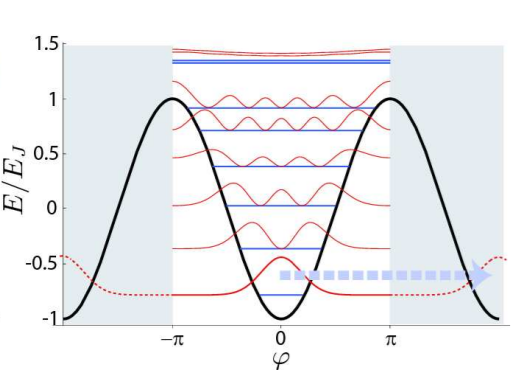
\includegraphics[width=0.5\textwidth]{pic/transmon/jj5.png}
\caption{Cosine potential with eigenenergies and squared moduli of the eigenfunction.Picture from \href{https://doi.org/10.1103/PhysRevA.76.042319}{Koch et al. PRA 2007}}
\label{fig:transmon2}
\end{figure}

This important condition allows us to approximate cosine potential as 
\begin{equation}
    -E_Jcos(\hat{\delta}) \simeq -E_J + E_J\frac{\hat{\delta}^2}{2} -E_J\frac{\hat{\delta}^4 }{4!} + ...
\end{equation}
So, supposing $n_g \simeq 0$, we could approximate the Hamiltonian of qe \ref{HamiltonianJJ} as
\begin{equation}
    H \simeq 4E_c\hat{n}^2 + E_J\frac{\hat{\delta}^2}{2} -E_J\frac{\hat{\delta}^4 }{4!}
\end{equation}
and by redefining the operators $\hat{n}$ and $\hat{\delta}$ as
\begin{equation}
    \begin{split}
        \hat{n} = n_0(\hat{a} + \hat{a}^+)\\
        \hat{\delta} = i\delta_{0}(\hat{a}^+ - \hat{a})
    \end{split}
\end{equation}
we could obtain the final form of the Hamiltonian (see Appendix)
\begin{equation}
\label{HamiltonianSimplified}
    \begin{split}
        H = \hbar\omega\hat{a}^+\hat{a} + \frac{\hbar\alpha}{2}(\hat{a}^+)^2(\hat{a})^2\\ \\
        \omega = \sqrt{8E_CE_J} - E_C \\  \alpha = \frac{E_C}{\hbar} 
        \end{split}
\end{equation} 

\section{Squids: a couple of words}
Up to this moment we have only analysed what happens to a single Josephsonn junction circuit. However, as it could be seen from eq. \ref{HamiltonianSimplified} the value of $\omega$ is depending on $E_C$ and $E_J$ which are fixed once we produce the junction. This situation presents two back-draws:
\begin{itemize}
    \item $\omega$ could not be precisely determined since production processes does not allow us to have enough precision nor over $E_C$ nor $E_J$ 
    \item $\omega$ can not be dynamically changed and this would be problematic for performing two qubit gates
\end{itemize}
In order to overcome these limitations Squids (Superconducting Quantum Interference Devices) were introduced. Fig. illustrates what is the circuital structure of Squids: they are composed by two, usually identical, Josephson junction in parallel. This introduces a superconducting loop into the circuit whose properties could be controlled with the aid of an external magnetic field $\Vec{B}$.
If we consider the flux associated to the closed path composed by the two junctions we could write:
\begin{equation}
    \hat{\phi_1}-\hat{\phi_2} +\frac{\Phi_{ext}}{\phi_0} = 2\pi m
\end{equation}
with $\phi_{1,2}$ the phase associated to each junction respectively, $\Phi_{ext}$ the flux of the external magnetic field through the two junction closed path, $\phi_0$ the quantum flux and $m \in \mathbb{Z}$.
Through some more detailed calculations it would be possible to show that it is possible to obtain a system that behaves like a single junction and that has a different tunneling Hamiltonian  
\begin{equation}
\begin{split}
    H_J = -2E_J|cos(f/2)|cos(\hat{\phi})\\ \\
    f = \Phi_{ext}/\phi_0\\
    \hat{\phi} = \frac{\hat{\phi_1} +\hat{\phi_2}}{2}
    \end{split}
\end{equation}


It is important to notice that now the tunneling energy $E_J\prime$ could be tuned at will by just changing the external flux that goes through the junction loop:
\begin{equation}
    E_J\prime = E_J|cos(f/2)|
\end{equation}
So Squids are able to guarantee more flexibility and tunability in situ also while the experiment is in progress

\begin{figure}[h]
\centering
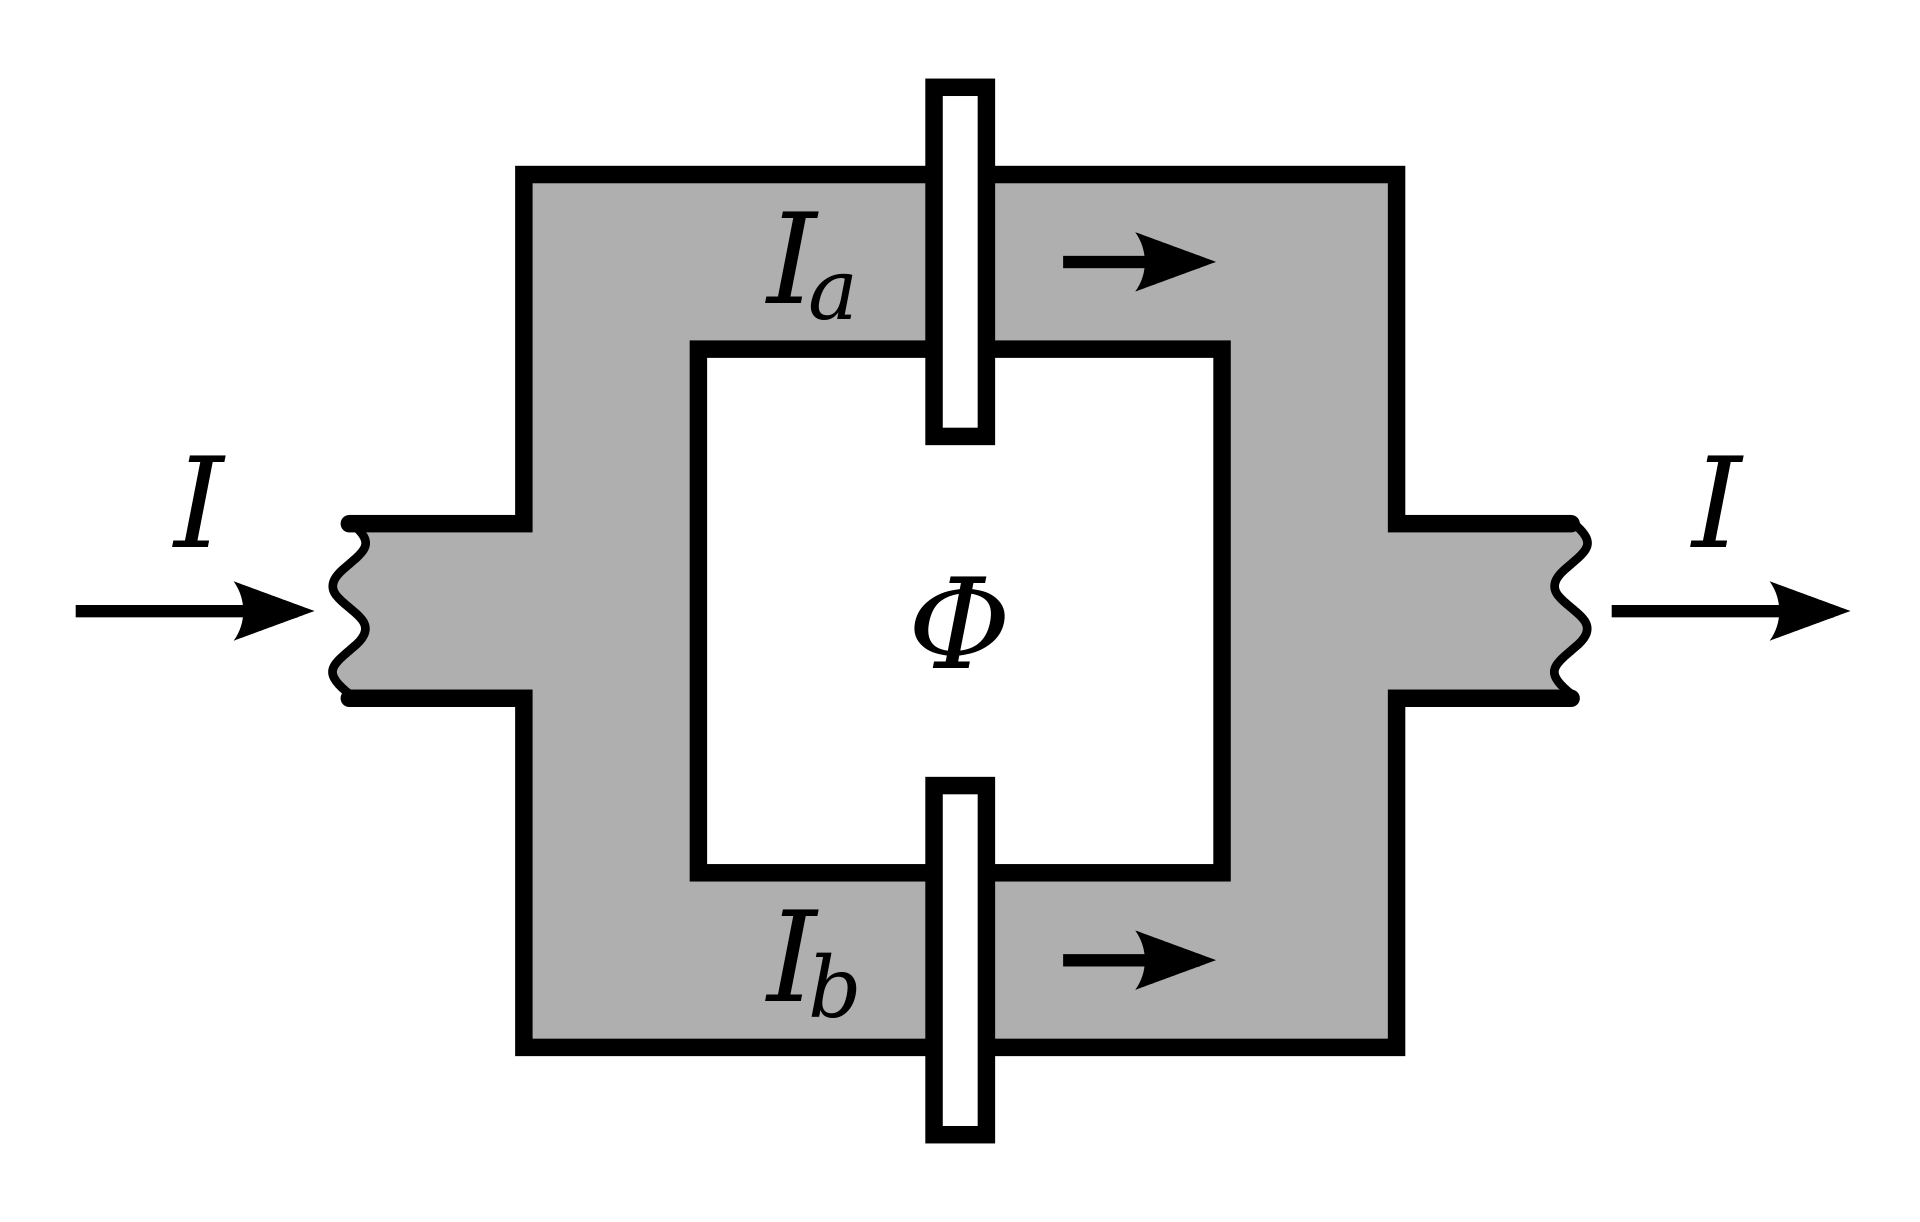
\includegraphics[width=0.3\textwidth]{pic/transmon/squid1.png}
%\caption{SQUID structure from \hyperlink{https://it.wikipedia.org/wiki/SQUID}{Wikipedia} }
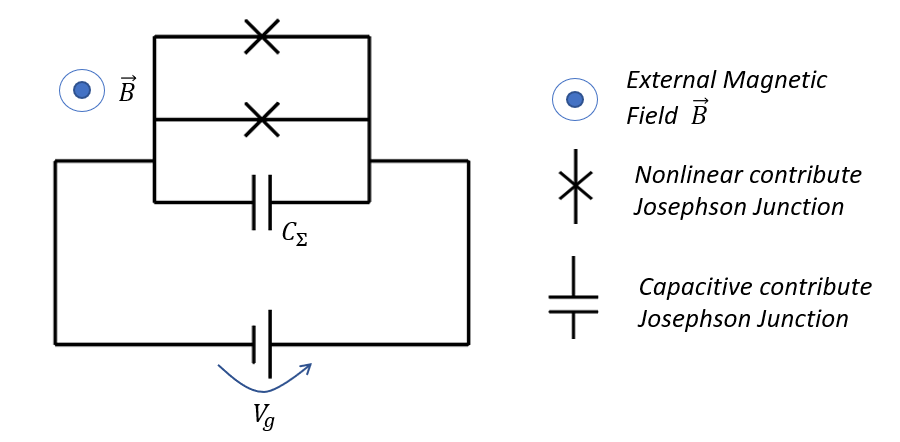
\includegraphics[width=0.7\textwidth]{pic/transmon/squid2.png}
\caption{SQUID circuital sketch}
\label{fig:squid1}
\end{figure}

\section{Transmon qubit in a 3d cavity}
After introducing, transmon qubit Hamiltonian let's have a look at the practical realization that was chosen for this project. In order to simplify as mushc as possible the practical implementation of the device it was chosen to produce a transomn qubit in a 3d cavity. The main structure is shown in fig. \ref{}. We can see:
\begin{itemize}
    \item the transmon chip deposited over a sapphire substrate
    \item the electromagnetic cavity 
\end{itemize}
The cavity is implemented for trapping electromagnetic fields inside the cavity. We can study the interaction of the qubit with the stationary electromagnetic modes in a really controlled fashion and achieve particular working conditions as the dispersive regime. Let's focus now on the transmon chip.
\subsection{Transmon}
A more detailed structure of the transmon chip could be seen in fig. 
It shows a Squid structure (two Josephson Junction in parallel) connected to a two extremal conductive pads called respectively 'Island' and 'Reservoir' also made by the same superconductive material used for the josepshon junction. The presence of the pads is necessary as:
\begin{itemize}
    \item it increases the dipole associated to the transmon which contributes to a stronger coupling with the electormagnetic modes
    \item it increase the total capacitance of the qubit $C_{\Sigma}$ and so it contributes entering \footnote{Remember than $E_C = \frac{e^2}{2C_{\Sigma}}$ so as long $C_{\Sigma}$ increases $E_C$ decreases and we enter a 'deeper' transmon regime ($E_J/E_C \gg 1$) the strong coupling regime}
\end{itemize}
Let's first focus on the capacitance calculations and circuital structure which is shown in picture \ref{}. Notice that since the transmon is inserted inside a 3d electromagnetic cavity we have to consider also the capacitive interaction between the two. The complete effective capacitance will then be:
\begin{equation}
C_{\Sigma} = 2C_J + C_{I-R} + \left(\frac{1}{C_{R-C}} + \frac{1}{C_{I-C}}\right)^{-1}
\end{equation}
where $C_J$ is the Josephson junction capacitance, $C_{I-R}$ the capacitance between the Island and Reservoir, $C_{R-C}$ the capacitance between the Reservoir pad and the cavity, $C_{I-C}$ the capacitance between the island and cavity.\\
\par
Now let's have a look to dipole calculation. Since the dimensions ($~\mu m$)of the transmon are very small if compared with the cavity ones ($~mm$) we could consider the Electric field to be constant across all the qubit. Let's suppose $E(y) = E_0$ is parallel to the pads as represented in fig. Now we could also associate a potential to it, namely, $V(\vec(r)) = -E_0\cdot y$. The electric field induces a charge with the same modulus but opposite sign, over the transmon islands and reservoir$Q = - Q_{r} = Q_I$ We could then write the interaction Hamiltonian as:
\begin{equation}
    H_{int} = \int_{V} \rho(\vec{r})\,V(\vec{r})\,d\vec{r} = -E_0\, Q\, d_{t}
\end{equation}
where $V$ is the volume of the transmon, $\rho(\vec{r})$ is the charge density defined over all the transmon volume, Q is the total charge $d_{t}$ is the effective distance associated to the transmon and $Qd_{t}$ the effective dipole.
It should be noted that in this analysis we did not consider the presence of the two Josephson junctions. This is mainly due to the difficulty arisen in simulating the charge distribution over the Josephson junction. It would be possible to estimate roughly the effect of the junction with the following formula:
\begin{equation}
    d_t\prime = \frac{Q_J\,d_J+Q\,d_t}{Q_J + Q}
\end{equation}
with $Q_J$  and $d_J$the charge and effective distance associated to the junction. We performed some calculation starting from cad simulation result and it was possible to see that the effect of the junctions is really negligible.
We could finally write the quantum transmon Hamiltonian as:
\begin{equation}
    H_{int} =-\hat{E_0} \, \hat{Q} \, d_t = E_0\,(\hat{a} + \hat{a}^+)\, Q\, d_t\,\frac{\hat{b}^+- \hat{b}}{\sqrt{2}} = \hbar \sum_{i,j} g_{ij} \ket{i}\bra{j}(\hat{a} + \hat{a}^+)
\end{equation}
where $$\hat{Q} = Q\,\frac{\hat{b}^+- \hat{b}}{\sqrt{2}} = i\left(\frac{E_J}{8E_C}\right)^{1/4}\frac{\hat{b}^+- \hat{b}}{\sqrt{2}}$$ is the quantum charge operator, $$\hat{E}=E_0\,(\hat{a} + \hat{a}^+)$$ the electric field operator and $\ket{i}$ indicates a generic transmon level.
It is interesting to notice that
\begin{equation}
    \begin{split}
        \hbar\,g_{ij} = E_0\,Q\,d_t\,\bra{i}\left(\frac{\hat{b}^+- \hat{b}}{\sqrt{2}}\right)\ket{j}
    \end{split}
\end{equation}
By performing more detailed calculation \footnote{For acquiring a deeper insight over this section consult \hyperlink{https://arxiv.org/pdf/cond-mat/0703002.pdf}{Koch et al.}} in the large transmon limit ($ E_J/E_C \gg 1$) it is possible to obtain
\begin{equation}
    \begin{split}
        |\bra{j+1}\hat{n}\ket{j}| \approx \sqrt{\frac{j+1}{2}}\left(\frac{E_J}{8E_C}\right)^{1/4}\\
        |\bra{j+k}\hat{n}\ket{j}| \rightarrow 0  
    \end{split}
\end{equation}
So supposing that we have can have dipole transition only among subsequent levels and considering only the two fundamental levels of the transmon as $\ket{g} \: \ket{e}$ we could write
\begin{equation}
    H_{qubit} = \hbar\, \omega_{eg}\, \hat{a}^+\hat{a} + \hbar\, g_{eg}\, \hat{\sigma_x}\, (\hat{a} + \hat{a}^+)
\end{equation}
The practical calculations of both dipole and capacity are discussed in next chapters.

\chapter{3D Cavity}
%==========================
\section{Maxwell's equation}

\section{Rectangular cavity}

\section{Cylindrical cavity}

\section{Pure coaxial cavity}

\section{Combination cavity }
\subsection{Mode Analysis}
\subsection{Frequency shift due to coupling}
\subsection{Radiation power through opening cavity}

\section{Purcell filter for coaxial cavity}
\subsection{Coupling between cavities}
\subsubsection{Merged cavity and its problems}
\subsubsection{Coaxial coupling line (referring to University of California, Merged study)}
\subsection{Asymmetric design}
\subsection{Mode analysis for two cavities}

\subsubsection{Derivation}

Instead of driving our system with an external frequency source added to the readout resonator, we switch to the formalism where the input signal is fed in through transmission line, which is the case of our system. We use $b_{in}$ to denote amplitude of input signal from transmission line to Purcell filter. This result in
\\
\begin{equation} \begin{split}
	\dot \alpha &= - i \Delta_{rd} \alpha - i G \beta \\
	\dot \beta &= -i \Delta_{fd} \beta - i G^* \alpha - \frac{\kappa}{2} \beta + \sqrt{\kappa} b_{in}
\end{split} \end{equation}
\\
In the steady state, $\dot \alpha = \dot \beta = 0$. This yields
\\
\begin{equation} \begin{split}
	0 &= - i \Delta_{rd} \alpha - i G \beta \\
	0 &= -i \Delta_{fd} \beta - i G^* \alpha - \frac{\kappa}{2} \beta + \sqrt{\kappa} b_{in}
\end{split} \end{equation}
\\
We can easily obtain realtion between $\alpha$ and $\beta$
\\
\begin{equation}
	\alpha = -\frac{G}{\Delta_{rd}} \beta
	\label{eq:rela_alphabeta}
\end{equation}
Substitute Eq\ref{eq:rela_alphabeta} back to the steady state equation for $\beta$, we obtain its steady state solution
\\
\begin{equation}
	\beta = \frac{\sqrt{\kappa}b_{in}}{\frac{\kappa}{2} + i (\Delta_{fd} - \frac{|G|^2}{\Delta_{rd}})}
	\label{eq:steadyStateBeta}
\end{equation}
\\
Boundary conditon of the input-output theory yields
\\
\begin{equation}
	\sqrt{\kappa} \beta = b_{in} + b_{out}
	\label{eq:boundaryCondition}
\end{equation}
\\
Substituting Eq\ref{eq:boundaryCondition} to the definition of the network parameter $S_{11}$ will lead to
\\
\begin{equation}
	S_{11} = \frac{b_{out}}{b_{in}} = \frac{\sqrt{\kappa}\beta}{b_{in}} - 1
\end{equation}
\\
Combining Eq\ref{eq:steadyStateBeta}, we obtain
\\
\begin{equation}
	S_{11} = \frac{\kappa}{\frac{\kappa}{2} + i (\Delta_{fd} - \frac{|G|^2}{\Delta_{rd}})} - 1
\end{equation}
\\
Through simple calculation we will find $S_{11}$ has rather simple form
\\
\begin{equation}
	S_{11} = \frac{(\frac{\kappa}{2})^2 - (\Delta_{fd} - \frac{|G|^2}{\Delta_{rd}})^2}{(\frac{\kappa}{2})^2 + (\Delta_{fd} - \frac{|G|^2}{\Delta_{rd}})^2} + i \frac{-2(\frac{\kappa}{2})(\Delta_{fd} - \frac{|G|^2}{\Delta_{rd}})}{(\frac{\kappa}{2})^2 + (\Delta_{fd} - \frac{|G|^2}{\Delta_{rd}})^2}
\end{equation}
\\
We can verify that the absolute value of $S_{11}$ is always $1$. This coincide with our intuition for the system: since no energy is allowed to leak out through readout resonator, the only way for the energy input to go out is through output coupling of the Purcell filter. At the steady state, amplitude of signal input should be equal to that of output (otherwise the total energy stored in the system is changed and this will not be steady state any more). Now we only look into the imaginary part of $S_{11}$. It deterministically give the experssion of the phase of $S_{11}$
\\
\begin{equation}
	\mathrm{sin}(\phi) = \mathrm{Im}[S_{11}]
\end{equation}
\\
\begin{equation}
	\mathrm{Im}[S_{11}] = \frac{-2(\frac{\kappa}{2})(\Delta_{fd} - \frac{|G|^2}{\Delta_{rd}})}{(\frac{\kappa}{2})^2 + (\Delta_{fd} - \frac{|G|^2}{\Delta_{rd}})^2}
	\label{eq:ImaginaryS11}
\end{equation}
\\
Eq\ref{eq:ImaginaryS11} has the form of dispersive lineshape. To continue discovering $\mathrm{Im}[S_{11}]$ we denote following substitution
\\
\begin{equation}
	f(\Delta) = \Delta_{fr} + \Delta - \frac{|G|^2}{\Delta}
\end{equation}
\\
In which $\Delta_{fr} \equiv \omega_f - \omega_r$ equals to the detuning between two resonators, while $\Delta \equiv \Delta_{rd}$ for the simplicity of notation. $\mathrm{Im}[S_{11}]$ then becomes a dispersive function with respect to $f(\Delta)$
\\
\begin{equation}
	\mathrm{Im}[S_{11}] = - \frac{2 (\frac{\kappa}{2}) f(\Delta)}{(\frac{\kappa}{2})^2 + f(\Delta)^2}
\end{equation}
\\
Its intersection with $x$ axis appears under the condition $f(\Delta) = 0$, this leads to
\\
\begin{equation}
	\Delta_{fr} + \Delta - \frac{|G|^2}{\Delta} = 0
	\label{eq:eqForCentralFreq}
\end{equation}
\\
Solving Eq\ref{eq:eqForCentralFreq} gives us values of two mode frequency
\\
\begin{equation} \begin{split}
	\Delta_1 = -\frac{1}{2} \Delta_{fr} + \frac{1}{2} \sqrt{\Delta_{fr}^2 + 4|G|^2} \\
	\Delta_2 = -\frac{1}{2} \Delta_{fr} - \frac{1}{2} \sqrt{\Delta_{fr}^2 + 4|G|^2}
	\label{eq:centerSolution}
\end{split} \end{equation}
\\
Extremum of $\mathrm{Im}[S_{11}]$ gives us information of effective linewidth of the system \footnote{Depending on different measurement of linewidth, there might be a difference of a constant coefficient. However, this should not harm our discussion.}. This happens when
\\
\begin{equation}
	\Delta_{fr} + \Delta - \frac{|G|^2}{\Delta} = \left|\frac{\kappa}{2}\right|
\end{equation}
\\
This lead to four roots for $\Delta$
\begin{equation} \begin{split}
	\Delta_1^1 = -\frac{1}{2} \Delta_{fr} + \frac{\kappa}{4} + \frac{1}{2}\sqrt{\left(\Delta_{fr} - \frac{\kappa}{2}\right)^2 + 4|G|^2} \\
	\Delta_1^2 = -\frac{1}{2} \Delta_{fr} - \frac{\kappa}{4} + \frac{1}{2}\sqrt{\left(\Delta_{fr} + \frac{\kappa}{2}\right)^2 + 4|G|^2} \\
	\Delta_2^1 = -\frac{1}{2} \Delta_{fr} + \frac{\kappa}{4} - \frac{1}{2}\sqrt{\left(\Delta_{fr} - \frac{\kappa}{2}\right)^2 + 4|G|^2} \\
	\Delta_2^2 = -\frac{1}{2} \Delta_{fr} - \frac{\kappa}{4} - \frac{1}{2}\sqrt{\left(\Delta_{fr} + \frac{\kappa}{2}\right)^2 + 4|G|^2}
	\label{eq:peakSolution}
\end{split} \end{equation}
\\
In principle with Eq\ref{eq:centerSolution} and Eq\ref{eq:peakSolution} one should be able to solve parameters of interest, including $\Delta_{fr}$, $\kappa$ and $G$. Note that in the derivation we still haven't applied any approximation, this should work for the general case.

\subsubsection{Discussion on the large detuning case}

We assumme that we have obtained a spectrum where the Purcell fiter and the readout resonator is largely detuned. Also if we would like to observe a clear spectrum during simulation, we have to make sure that the decay rate $\kappa$ is small enough so that we can setlength two peaks. As a result, we come to a condition that $\kappa / 2 \ll |G|, \Delta_{fr}$, and $|G|$ is significantly smaller than $\Delta_{fr}$. This leads us to some simplicity during discussion. 

\begin{figure}[htbp]
     \centering
     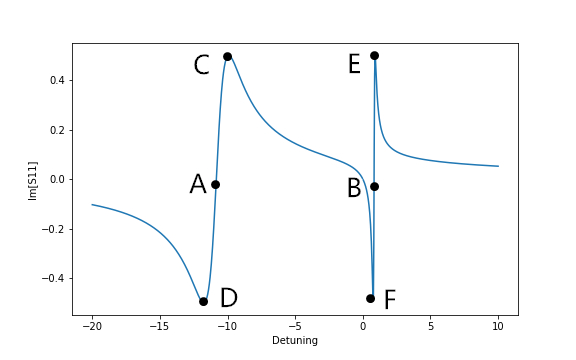
\includegraphics[width=11cm]{pic/3D_cavity/3D_twoCavityResonance.jpg}
     \caption{Dependence of inaginary part of $S_{11}$ on the detuning $\Delta$}
     \label{fig:ImS11}
\end{figure}

Fig\ref{fig:ImS11} is plotted under the condition above. Point A,B in the figure corresponds to two roots for the zero point of $S_{11}$, i.e. $\Delta_2, \Delta_1$ in the text above. Point C, D corresponds to the two peaks sitting around $\Delta_2$, which is the $\Delta_2^1, \Delta_2^2$ in the previous text. The same interpretation also applies to point E, F. From this correspondency we can tell that it is fair to say differnce $|\Delta_1^1 - \Delta_1^2|$ and $|\Delta_2^1 - \Delta_2^2|$ can be interpreted as linewidth of the cavity.

By applying large detuning condition, we can obtain approximation
\\
\begin{equation} \begin{split}
	& \sqrt{\left( \Delta_{fr} \pm \frac{\kappa}{2}\right)^2 + 4 |G| ^ 2} \\
	= & \sqrt{ \Delta_{fr}^2 + \left(\frac{\kappa}{2}\right)^2 \pm 2 \Delta_{fr} \frac{\kappa}{2} + 4 |G| ^ 2} \\
	\approx & \sqrt{ \Delta_{fr}^2 \pm 2 \Delta_{fr} \frac{\kappa}{2} + 4 |G| ^ 2} \\
	\approx & \sqrt{ \Delta_{fr}^2 + 4 |G| ^ 2} \pm \frac{\Delta_{fr}}{\sqrt{ \Delta_{fr}^2 + 4 |G| ^ 2}} \frac{\kappa}{2}
\end{split} \end{equation}
\\
This leads to approximate value of extremum points
\begin{equation} \begin{split}
	\Delta_1^1 = -\frac{1}{2} \Delta_{fr} + \frac{1}{2}\sqrt{\Delta_{fr}^2 + 4|G|^2}  + \frac{\kappa}{4} - \frac{\Delta_{fr}}{\sqrt{ \Delta_{fr}^2 + 4 |G| ^ 2}} \frac{\kappa}{4} \\
	\Delta_1^2 = -\frac{1}{2} \Delta_{fr} + \frac{1}{2}\sqrt{\Delta_{fr}^2 + 4|G|^2}  - \frac{\kappa}{4} + \frac{\Delta_{fr}}{\sqrt{ \Delta_{fr}^2 + 4 |G| ^ 2}} \frac{\kappa}{4} \\
	\Delta_2^1 = -\frac{1}{2} \Delta_{fr} - \frac{1}{2}\sqrt{\Delta_{fr}^2 + 4|G|^2}  + \frac{\kappa}{4} + \frac{\Delta_{fr}}{\sqrt{ \Delta_{fr}^2 + 4 |G| ^ 2}} \frac{\kappa}{4} \\
	\Delta_2^2 = -\frac{1}{2} \Delta_{fr} - \frac{1}{2}\sqrt{\Delta_{fr}^2 + 4|G|^2}  - \frac{\kappa}{4} - \frac{\Delta_{fr}}{\sqrt{ \Delta_{fr}^2 + 4 |G| ^ 2}} \frac{\kappa}{4}
\end{split} \end{equation}
\\
Under the condition where detuning is significantly larger than coupling strength, $\Delta_1$ represents the solution where $\Delta_{rd}$ is small. Thus, we can see it as shifted readout cavity mode. The mode lindewidth
\\
\begin{equation}
	\frac{\delta \omega_1}{2} = |\Delta_1^1 - \Delta_1^2| = \left (1 - \frac{\Delta_{fr}}{\sqrt{ \Delta_{fr}^2 + 4 |G| ^ 2}} \right) \frac{\kappa}{2}
\end{equation}
\\
We can see that the shifted mode gained a finite linewidth due to its hyberdization with leaky Purcell filter mode. Nevertheless, the linewidth is suppressed by the large drtuning. The same interpretation also works for shifted Purcell filter mode
\\
\begin{equation}
	\frac{\delta \omega_2}{2} = |\Delta_2^1 - \Delta_2^2| = \left (1 + \frac{\Delta_{fr}}{\sqrt{ \Delta_{fr}^2 + 4 |G| ^ 2}} \right) \frac{\kappa}{2}
\end{equation}
\\
Which means that shifted Purcell filter mode endures a reduction in the linewidth. If the ratio $\Delta_{fr}/|G|$ goes to infinitely large, two cavity will become completely independent, $\delta \omega_1 \approx 0, \delta \omega_2 \approx \kappa$. This result coincide with our intuition.

It is worthwhile to note that we also obtained relationship
\begin{equation}
	\Delta_1 + \Delta_2 = - \Delta_{fr}
	\label{eq:centerConserved}
\end{equation}
and
\begin{equation}
	\delta \omega_1 + \delta \omega_2 = \kappa
	\label{eq:linewidthConserved}
\end{equation}
Eq\ref{eq:centerConserved} means that the numerical average of two mode frequency is conserved, Eq\ref{eq:linewidthConserved} means that the total linewidth is conserved.

\subsection{Purcell decay rate and readout cavity response}
\chapter{Input-output coupling for 3D cavity}
\section{General wave guide equations}
\section{Circular wave guide (TE, TM mode)}
\section{Coaxial wave guide (TEM, TE, TM mode)}
\section{Boundary condition of evanescent coupling}
\section{Coupling between wave guide and cavity mode}
\section{Quantized input-output coupling theory}
\chapter{Different Reset schemes and their expectations}

\section{Pumping Reset Scheme}
\subsection{Intuition behind scheme}



\section{Master Equation Formalism}
The crux of the quantum information processing is to understand the sources of the dissipation for possible remedies. However, the complexity of the interaction between the quantum system of interest and the surrounding environment render a general and assumption-free analysis intractable. In the closed system point of view, the result of the interaction between system and environment is a non-unitary evolution of the system's degrees of freedom, whose evolution can be modelled with stochastic wavefunction description \cite{smqo1}. In this description, the wavefunction of the system discovers one one the possible trajectories in its phase space, which is corresponding what could be observed in a single experimental run. As its name suggesting, this process is a non-deterministic process in which no deterministic control can be established over.

\vspace{2 mm}

On the other hand, under certain assumptions, the evolution of the closed system can be described by master equations \cite{davies}. In usual cases, the number of degrees of freedom in environment is huge such that the information leaked from the close system to environment cannot flow back to the system in any finite time, i.e. whenever the environment interacts with the closed system, the obtained information is quickly forgotten by the environment  due very short self-correlation time \cite{ahn}. Furthermore, if the environment (or reservoir) is considered as a measurement device which continuously probes the closed system, the resulting dynamics can be described as an average realization of each possible individual trajectories in the phase space of the total system. Alongside with this, the interaction between the closed system and environment is weak, and further separability of density functions of closed system and environment, the overall dynamics of the system can be described by Lindblad master equation formalism\footnote{The intricacies of the derivation leading to Lindblad master equation will not be discussed in the remainder of the report; however, for more detailed analysis can be found in the seminal work of C.W. Gardiner and M.J Collett \cite{gardinercollet1985}, and also "Theory of quantum noise and decoherence" course of Tobias J. Osborne in Youtube.}: 

\begin{equation}
    \Dot{\rho} = -i[H,\rho] + \sum_{\i=1}^{m} \mathcal{D}[c_i]\pho
\end{equation}

where the Lindblad superoperator $\mathcal{D}$ is $\mathcal{D}[c]\rho = c\rho c^\dagger - \frac{1}{2}c^\dagger c \rho -\frac{1}{2} \rho c^\dagger c$, and $\rho$ is the density matrix of the closed system (i.e. the density matrix obtained after the reservoir is traced out).

Thus, to be able to see the evolution of the closed system's density, the Hamiltonian of the system, the form of the collapse operators regarding the various dissipation or decoherence channels and the initial condition of the density matrix are the only requirements. In the next section, the question regarding on how to simulate the system will be explained in the pumping reset scheme specific.


\section{Master Equation Simulation of Pumping Reset Scheme with QuTiP }

\maketitle
	
\subsection{Hamiltonian}

	\begin{equation} \label{eq:full_hamiltonian}
	\begin{split}
		H = \underbrace{\hbar \omega_{eg}b^\dagger b - \frac{\alpha}{2} b^\dagger b ^\dagger b b }_{\text{qubit hamiltonian}}+ \underbrace{\hbar \omega_{1} a ^ \dagger a}_{\text{cavity mode}} + \underbrace{\hbar \omega_{2} c ^\dagger c}_{\text{reset mode}} + \underbrace{\hbar \omega_{3} d ^\dagger d}_{\text{pump mode}} \\
		+\underbrace{\hbar  g_1(b^\dagger a + a ^\dagger b) + \hbar g_2(b^\dagger c + c^\dagger b) + \hbar g_3(b^\dagger d + d^\dagger b)}_{\text{interaction term}}.
    \end{split}
	\end{equation}

	By choosing this form of the Hamiltonian, the rotating wave approximation is already applied. On the other hand, the time dependence of the interaction term was not written explicitly in Eqn. \ref{eq:full_hamiltonian}. For the rest of the analysis, the Hamiltonian is parted into two parts, namely quadratic and quartic.
	
\vspace{3mm}

	Now we write down the quadratic term,
	\begin{equation} \label{eq:h2}
	\begin{split}
		h_2 = \hbar \omega_{eg}b^\dagger b + \hbar \omega_{1} a ^ \dagger a +\hbar \omega_{2} c ^\dagger c + \hbar \omega_{3} d ^\dagger d \\
		+\hbar  g_1(b^\dagger a + a ^\dagger b) + \hbar g_2(b^\dagger c + c^\dagger b) + \hbar g_3(b^\dagger d + d^\dagger b) 
    \end{split}
	\end{equation} 
	
	And quartic term of the Hamiltonian,
	
	\begin{equation}\label{eq:h4}
	h_4 =- \frac{\hbar \alpha}{2} b^\dagger b ^\dagger b b 
	\end{equation}

	It can be better illustrated if we display $h_2$ in matrix format,
	\begin{equation}
		\frac{h_2}{\hbar} = \begin{pmatrix} b^\dagger & a ^ \dagger & c^\dagger & d^\dagger \end{pmatrix}
		\begin{pmatrix}
		\omega_{ge} & g_1 & g_2 & g_3 \\
		g_1 & \omega_1 & 0 & 0 \\
		g_2 & 0 & \omega_2 & 0\\
		g_3 & 0 & 0& \omega_3
		\end{pmatrix}
		\begin{pmatrix} b \\ a \\ c  \\ d\end{pmatrix}
	\end{equation}


	To diagonalize $h_2$ we would like to calculate eigenvectors of the coefficient matrix. However, the root of a qubic equation is usually complicated, which leads to even more complex expression of eigenvectors. However, the detuning between the modes and the values of the coupling strengths allow neglecting the complicated higher order terms in the perturbative approach.

	Define the parameters
	\begin{equation}
		\begin{cases}
			\Delta_1 = \omega_1 - \omega_{ge} \\
			\Delta_2 = \omega_2 - \omega_{ge} \\
			\Delta_3 = \omega_3 - \omega_{ge} \\
			\varepsilon_1 = g_1 / \Delta_1 \\
			\varepsilon_2 = g_2 / \Delta_2 \\
			\varepsilon_3 = g_3 / \Delta_3
		\end{cases}
	\end{equation}

	First-order correction to eigenvectors are
	\begin{equation} \label{eq:1st-order-correction}
		\Phi_i^1 = \sum _{j \neq i} \frac{\langle \Phi_j | V | \Phi_i \rangle}{E_j - E_i}
	\end{equation}

In this case, ${E_i}$ denotes diagonal elements of coefficient matrix, while ${V_{ij}}$ denotes off-diagonal elements. Substituting first-order correction to Eq\ref{eq:1st-order-correction}, we obtain new eigenvectors
\begin{equation}
	\begin{cases}
		\tilde{b} = b - \frac{g_1}{\Delta_1} a - \frac{g_2}{\Delta_2} c - \frac{g_3}{\Delta_3} d \\
		\tilde{a} = a + \frac{g_1}{\Delta_1} b \\
		\tilde{c} = c + \frac{g_2}{\Delta_2} b \\
		\tilde{d} = d + \frac{g_3}{\Delta_3} b
	\end{cases}
\end{equation}

Inverse the solution and we will get the first order correction on diagonalizing $h_2$
\begin{equation} \label{eq:diagonalize}
	\begin{cases}
		b = \tilde{b} + \frac{g_1}{\Delta_1} \tilde{a} + \frac{g_2}{\Delta_2} \tilde{c} +\frac{g_3}{\Delta_3} \tilde{d} \\
		a = \tilde{a} - \frac{g_1}{\Delta_1} \tilde{b} \\
		c = \tilde{c} - \frac{g_2}{\Delta_2} \tilde{b} \\
		d = \tilde{d} - \frac{g_3}{\Delta_3} \tilde{b}
	\end{cases}
\end{equation}

The substitution given in Eqn. \ref{eq:diagonalize} diagonalizes $h_2$ by cancelling the direct interaction term between the cavity modes and qubit mode and producing terms in $\mathcal{O}(\frac{g^2}{\Delta^2})$, which are negligible in the weak coupling and/or large detuning.  After the substitution, the quadratic part of the Hamiltonian becomes, 

\begin{equation} \label{eq:h2_bare_tilde}
    \frac{h_{2,bare}}{\hbar} = (\omega_{eg}-\frac{g_1^2}{\Delta_1}-\frac{g_2^2}{\Delta_2}-\frac{g_3^2}{\Delta_3})\tilde{b}^\dagger \tilde{b} + (\omega_1+\frac{g_1^2}{\Delta_1})\tilde{a}^\dagger \tilde{a}+ (\omega_2+\frac{g_2^2}{\Delta_2})\tilde{c}^\dagger \tilde{c} + (\omega_3+\frac{g_3^2}{\Delta_3})\tilde{d}^\dagger \tilde{d}
\end{equation}

In addition to terms in Eqn. \ref{eq:h2_bare_tilde}, this substitution introduces effective interaction term between readout and reset resonator and also effective driving terms for both resonators, which are mediated by qubit,

\begin{equation} \label{eq:h2_int_tilde}
    \frac{h_{2,int}}{\hbar} = \omega_{eg} \frac{g_1 g_2}{\Delta_1 \Delta_2}(\tilde{a}^\dagger \tilde{c} + \tilde{a} \tilde{c}^\dagger) + \omega_{eg} \frac{g_2 g_3}{\Delta_2 \Delta_3}(\tilde{c}^\dagger \tilde{d} + \tilde{c} \tilde{d}^\dagger) +\omega_{eg} \frac{g_1 g_3}{\Delta_1 \Delta_3}(\tilde{a}^\dagger \tilde{d} + \tilde{a} \tilde{d}^\dagger)
\end{equation}
Although the terms in Eqn. \ref{eq:h2_int_tilde} are rotating fast with compared to the timescale of interest, their coefficients are significant enough to affect the fidelity of reset process. Thus, they are taken into account in Lindblad master eqaution simulation. Next, we would like to substitute the corresponding terms in $h_4$ in order to get the corrections on state-depending frequency shift and two-photon process.

\begin{equation} \label{eq:h4-correction}
    \frac{h_4}{\hbar} = -\frac{\alpha}{2} (\tilde{b}^\dagger + \varepsilon_1 \tilde{a}^\dagger + \varepsilon_2 \tilde{c}^\dagger + \varepsilon_3 \tilde{d}^\dagger)^2 (\tilde{b} + \varepsilon_1 \tilde{a} + \varepsilon_2 \tilde{c} + \varepsilon_3 \tilde{d})^2
\end{equation}

The expansion of the Eqn. \ref{eq:h4-correction} contains 64 terms. After rotating wave approximation, considering the pumping mode as a coherent EM tone and ignoring the terms having the coefficient proportional to $\epsilon^3$ or higher, the number of terms in the quartic Hamiltonian is significantly reduced. First, let's focus on the terms corresponding to frequency shifts occurring qubit's transition frequency due to the EM modes coupled dispersively\footnote{Mode operators with tilde are written without tilde (i.e. $\tilde{O} \xrightarrow[]{} O$) to simplify the notation.},

\begin{equation} \begin{split}
	\chi_1 &= -2\alpha \varepsilon_1^2 b^\dagger b a^\dagger a \\
	\chi_2 &= -2\alpha \varepsilon_2^2 b^\dagger b c^\dagger c \\
	\chi_3 &= -2\alpha \varepsilon_3^2 \abs{\Omega_d}^2 b^\dagger b 
\end{split} \end{equation}

This corresponds to dispersive shift due to coupling between qubit and two quantized modes (the modes of readout and reset resonator), and one coherent EM field (pump mode). As we have already explained in the introduction, an effective two photon process can be engineered by choosing the frequency of the coherent field as,

\begin{equation} \begin{split}
 \omega_3 = \omega_2 - 2\tilde{\omega}_{eg} + \alpha 
\end{split} \end{equation}

where $\tilde{\omega}_{eg}$ is the renormalized transition frequency of the qubit after the effects of other modes are taken into account. Consequently, 
\begin{equation}
	H_{2-pho} = -\alpha\varepsilon_2\varepsilon_3(b^\dagger b^\dagger cd+bbc^\dagger d^\dagger)
\end{equation}

This term corresponds to two-photon interaction between qubit, resonator field and pump field. If we pump with coherent light field, we can substitute operator $d$ by $\Omega_d$ (assume $\Omega_d$ to be real).
\begin{equation}
	H_{2-pho} = -\alpha\varepsilon_2\varepsilon_3\abs{\Omega_d} (b^\dagger b^\dagger c e^{i\omega_3 t} + bbc^\dagger e^{-i\omega_3 t})
\end{equation}

The coefficient $\alpha\varepsilon_2\varepsilon_3\Omega_d$ represents the rate of this two-photon process. Since, the coefficients $\varepsilon_2$ and $\varepsilon_3$ are small numbers due to detuning, the drive strength should be high in order to observe the effect of the two-photon process, which is needed to pump the population in $\ket{f}$ level of the qubit to lossy cavity mode ($\hat{c}$). The other important term is the effective driving of the qubit by the pump mode ($\hat{d}$) due to its amplitude,

\begin{equation}
	H_{ind,dri} = -\alpha (2\varepsilon_3 b^\dagger b \abs{\Omega_d} + \varepsilon_3^3 \abs{\Omega_d}^3) (b^\dagger e^{i\omega_3 t} +b e^{-i \omega_3 t})
\end{equation}

As a result, the Hamiltonian of the system after the perturbative approach, 

\begin{equation}\begin{split}
   \frac{\mathcal{H}}{\hbar} = (\omega_{eg}-\frac{g_1^2}{\Delta_1}-\frac{g_2^2}{\Delta_2}-\frac{g_3^2}{\Delta_3})b^\dagger b + (\omega_1+\frac{g_1^2}{\Delta_1})a^\dagger a+ (\omega_2+\frac{g_2^2}{\Delta_2})c^\dagger c  \\
\omega_{eg} \frac{g_1 g_2}{\Delta_1 \Delta_2}(a^\dagger c + a c^\dagger) + \omega_{eg} \frac{g_2 g_3}{\Delta_2 \Delta_3}\abs{\Omega_d}(c^\dagger e^{i\omega_3 t} + c e^{-i\omega_3 t}) +\omega_{eg} \frac{g_1 g_3}{\Delta_1 \Delta_3}\abs{\Omega_d}(a^\dagger e^{i\omega_3 t}+ a e^{-i\omega_3 t}) \\
  -2\alpha \varepsilon_1^2 b^\dagger b a^\dagger a 
	 -2\alpha \varepsilon_2^2 b^\dagger b c^\dagger c 
	 -2\alpha \varepsilon_3^2 \abs{\Omega_d}^2 b^\dagger b \\
-\alpha\varepsilon_2\varepsilon_3\abs{\Omega_d} (b^\dagger b^\dagger c e^{i\omega_3 t} + bbc^\dagger e^{-i\omega_3 t})\\
-\alpha (2\varepsilon_3 b^\dagger b \abs{\Omega_d} + \varepsilon_3^3 \abs{\Omega_d}^3) (b^\dagger e^{i\omega_3 t} +b e^{-i \omega_3 t})
\end{split}
\end{equation}

\subsection{Collapse Operators}

In this section, the interaction between the close system comprised of qubit-cavity and the environment. In our system, the following decoherence and dissipation sources are taken into account:

\begin{itemize}
  \item Decay rate of the readout resonator: $\kappa_{read}$
  \item Decay rate of the reset resonator: $\kappa_{reset}$
  \item Decay rate of transmon in between $\ket{g}$ and $\ket{e}$: $\gamma_{1,ge}$
  \item Decay rate of transmon in between $\ket{e}$ and $\ket{f}$: $\gamma_{1,ef}$
  \item Pure dephasing rate of transmon in between $\ket{g}$ and $\ket{e}$: $\gamma_{\phi,ge}$
  \item Pure dephasing rate of transmon in between $\ket{e}$ and $\ket{f}$: $\gamma_{\phi,ef}$
\end{itemize}


\subsection{Form of the Master Equation}

As a result, the final form of the master equation becomes,

\begin{equation} \begin{split}
	\Dot{\rho} = -i[\hat{\mathcal{H}},\rho] + \kappa_{read}\mathcal{D}[\hat{a}]\rho +  \kappa_{reset}\mathcal{D}[\hat{c}]\rho  \\
	+(n_{th}+1)\gamma_{1,ge}\mathcal{D}[\ket{g}\bra{e}]\rho + n_{th} \gamma_{1,ge}\mathcal{D}[\ket{e}\bra{g}]\rho\\
	+\gamma_{1,ef}\mathcal{D}[\ket{e}\bra{f}]\rho  + n_{th} \gamma_{1,ef}\mathcal{D}[\ket{f}\bra{e}]\rho \\
	+ \frac{\gamma_{\phi,ge}}{2} \mathcal{D}[\ket{e}\bra{e}-\ket{g}\bra{g}]\rho + \frac{\gamma_{\phi,ef}}{2} \mathcal{D}[\ket{f}\bra{f}-\ket{e}\bra{e}]\rho
	\end{split}
\end{equation}

where $\mathcal{D}[\hat{O}] \bullet = \hat{O} \bullet \hat{O}^\dagger - \frac{1}{2}\left\{\hat{O}^\dagger \hat{O}, \bullet \right\}$ is the dissipation or decoherence superoperator, and $n_{th}$ is the thermal population of the transmon qubit in steady state. 

\section{QuTiP Simulation}

In this section, the simulation results of the Lindblad master equation for the Hamiltonian and collapse operators associated with the pumping reset scheme. In this simulation, we are considering the 7.4 GHz mode as the readout mode, and 18.75 GHz mode as the reset mode. The coupling strength between these modes and qubit are determined with the ANSYS simulations. On the other side, the qubit-related parameters are taken from Magnard et. al paper \cite{Magnard} given the fact that the design and fabrication of the qubit was cancelled due COVID-19 pandemic. 

\vspace{2 mm}

In this reset scheme, unlike Magnard et.al's approach, the pulse between $\ket{e}$ and $\ket{f}$ is a mere $\pi$-pulse without any optimization. The only control and optimization knob of this scheme is the duration and the frequency of the pumping pulse. Furthermore, since the frequency difference between $\ket{g,1}$ and  $\ket{f,0}$ states are depending on the pump frequency and pulse strength, it is analytically challenging to find the correct pulse parameters. Therefore, the first simulation aims to determine the frequency of the pumping pulse for a fixed pulse duration (150 ns) which yields the best reset fidelity, 

\begin{figure}[h]
    \centering
    \includegraphics[width=1\textwidth]{pic/different_reset_schemes/qubit_pop_max_reset_pop_to_det_freq.eps}
    \caption{a) The population of the qubit and b) the maximum value of the population of the reset resonator after the system is driven by 150 ns pulse with different frequencies.}
    \label{fig:freq_sweep_qubit_reset_max}
\end{figure}


\begin{figure}[h]
    \centering
    \includegraphics[width=1\textwidth]{pic/different_reset_schemes/gef_pop.eps}
    \caption{The population in $\ket{g}$, $\ket{e}$ and $\ket{f}$ state after the system is driven by 150 ns pulse with different frequencies.}
    \label{fig:freq_sweep_gef}
\end{figure}


In the first subplot in Fig. \ref{fig:freq_sweep_qubit_reset_max}, where the overall qubit population is depicted, the population is plummeting down near to zero for the frequency of 7.10 GHz, while the population in the reset resonator reaches its peak for this particular frequency, which signals that the population transfer from $\ket{f,0}$ to $\ket{g,1}$ is maximized. Furthermore in Fig. \ref{fig:freq_sweep_gef}, one can see that the population in $\ket{f}$ state is drained to $\ket{g}$ state but not to $\ket{e}$, which is evident from the fact that the population in $\ket{e}$ state is also attaining its lowest value.


\vspace{2 mm}

The next parameter to be simulated is the duration of the pulse. In the previous analysis, for a fixed pulse duration, which is 150 ns, the frequency difference between the states $\ket{f,0}$ and $\ket{g,1}$ was determined. However, the duration of the pulse is the other integral part of the Rabi flip between these states, since any trajectory on Bloch sphere is determined both frequency, coupling strength and duration of the driving term.  


For determining the pulse duration which yield near-perfect population transfer from the qubit subspace to reset resonator subspace, the population of the qubit states are investigated under different pulse durations ranging from 100 to 200 ns. In the simulations, the overall evolution time is set to 500 ns.



\begin{figure}[h!]
    \centering
    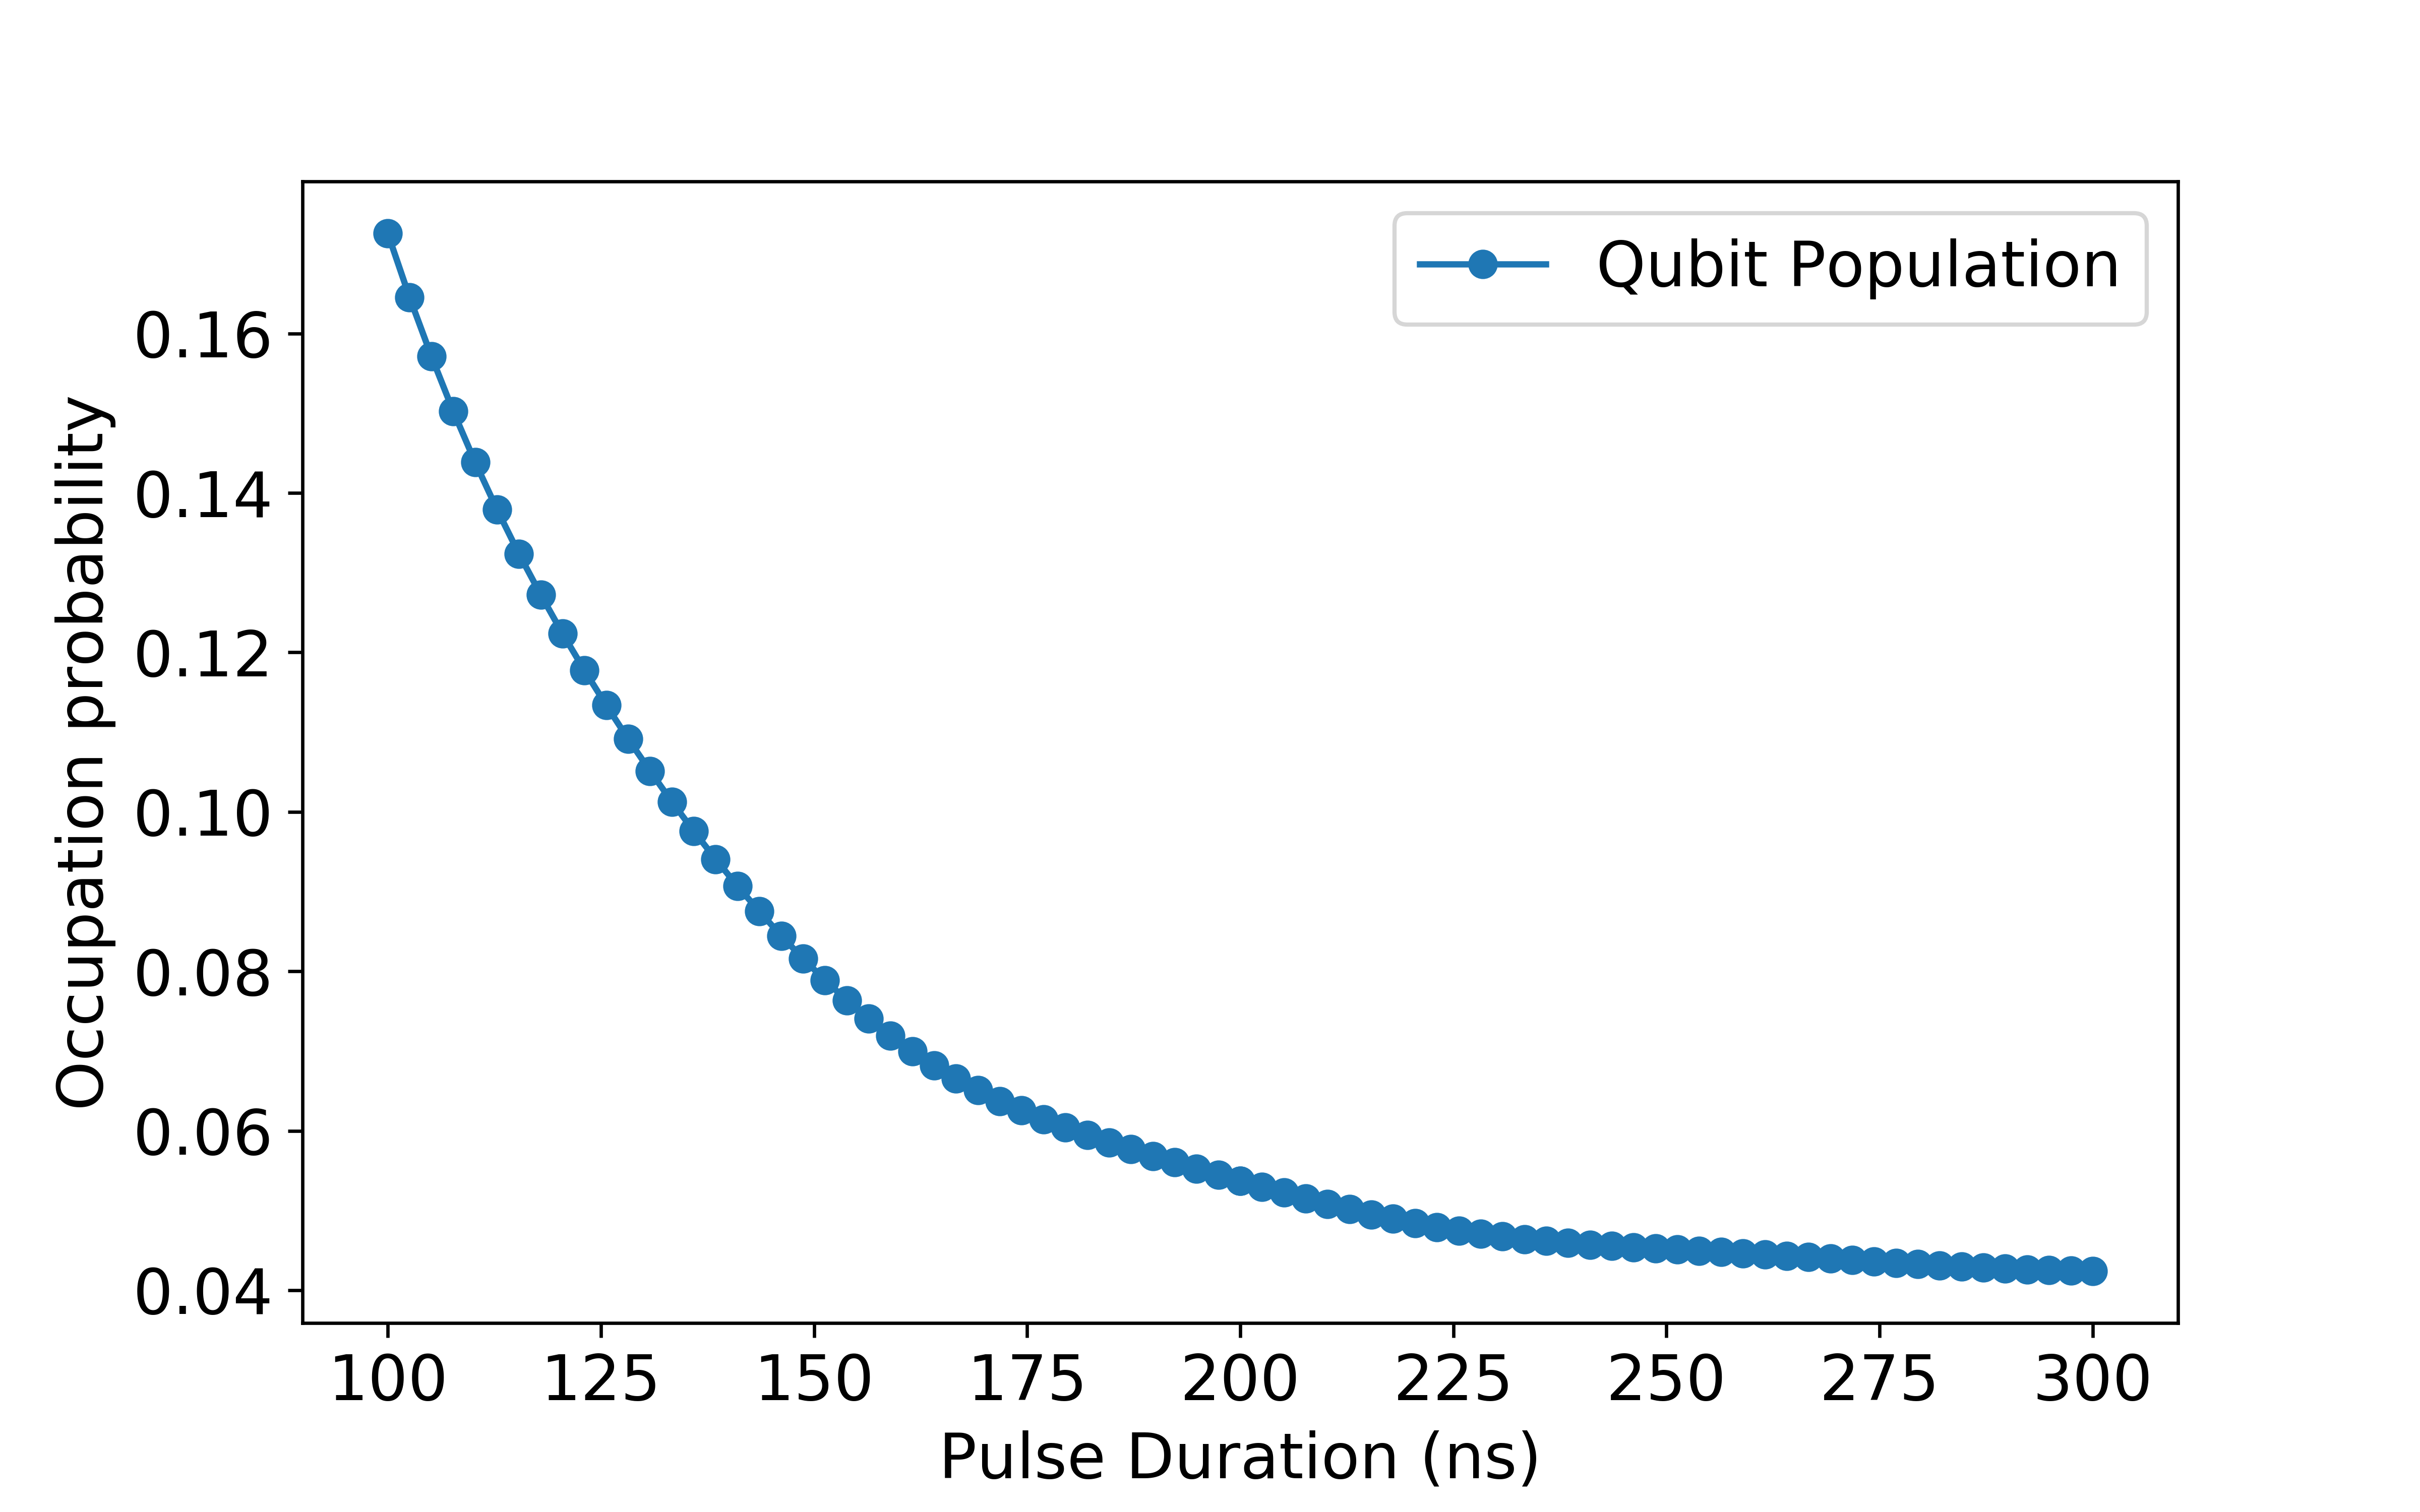
\includegraphics[width=0.6\textwidth]{pic/different_reset_schemes/qubit_pop_710_tau_sweep_100_300.png}
    \caption{The qubit and reset resonator population for pulse duration between 100 to 300 ns.}
    \label{fig:tau_sweep_qubit}
\end{figure}

\begin{figure}[h!]
    \centering
    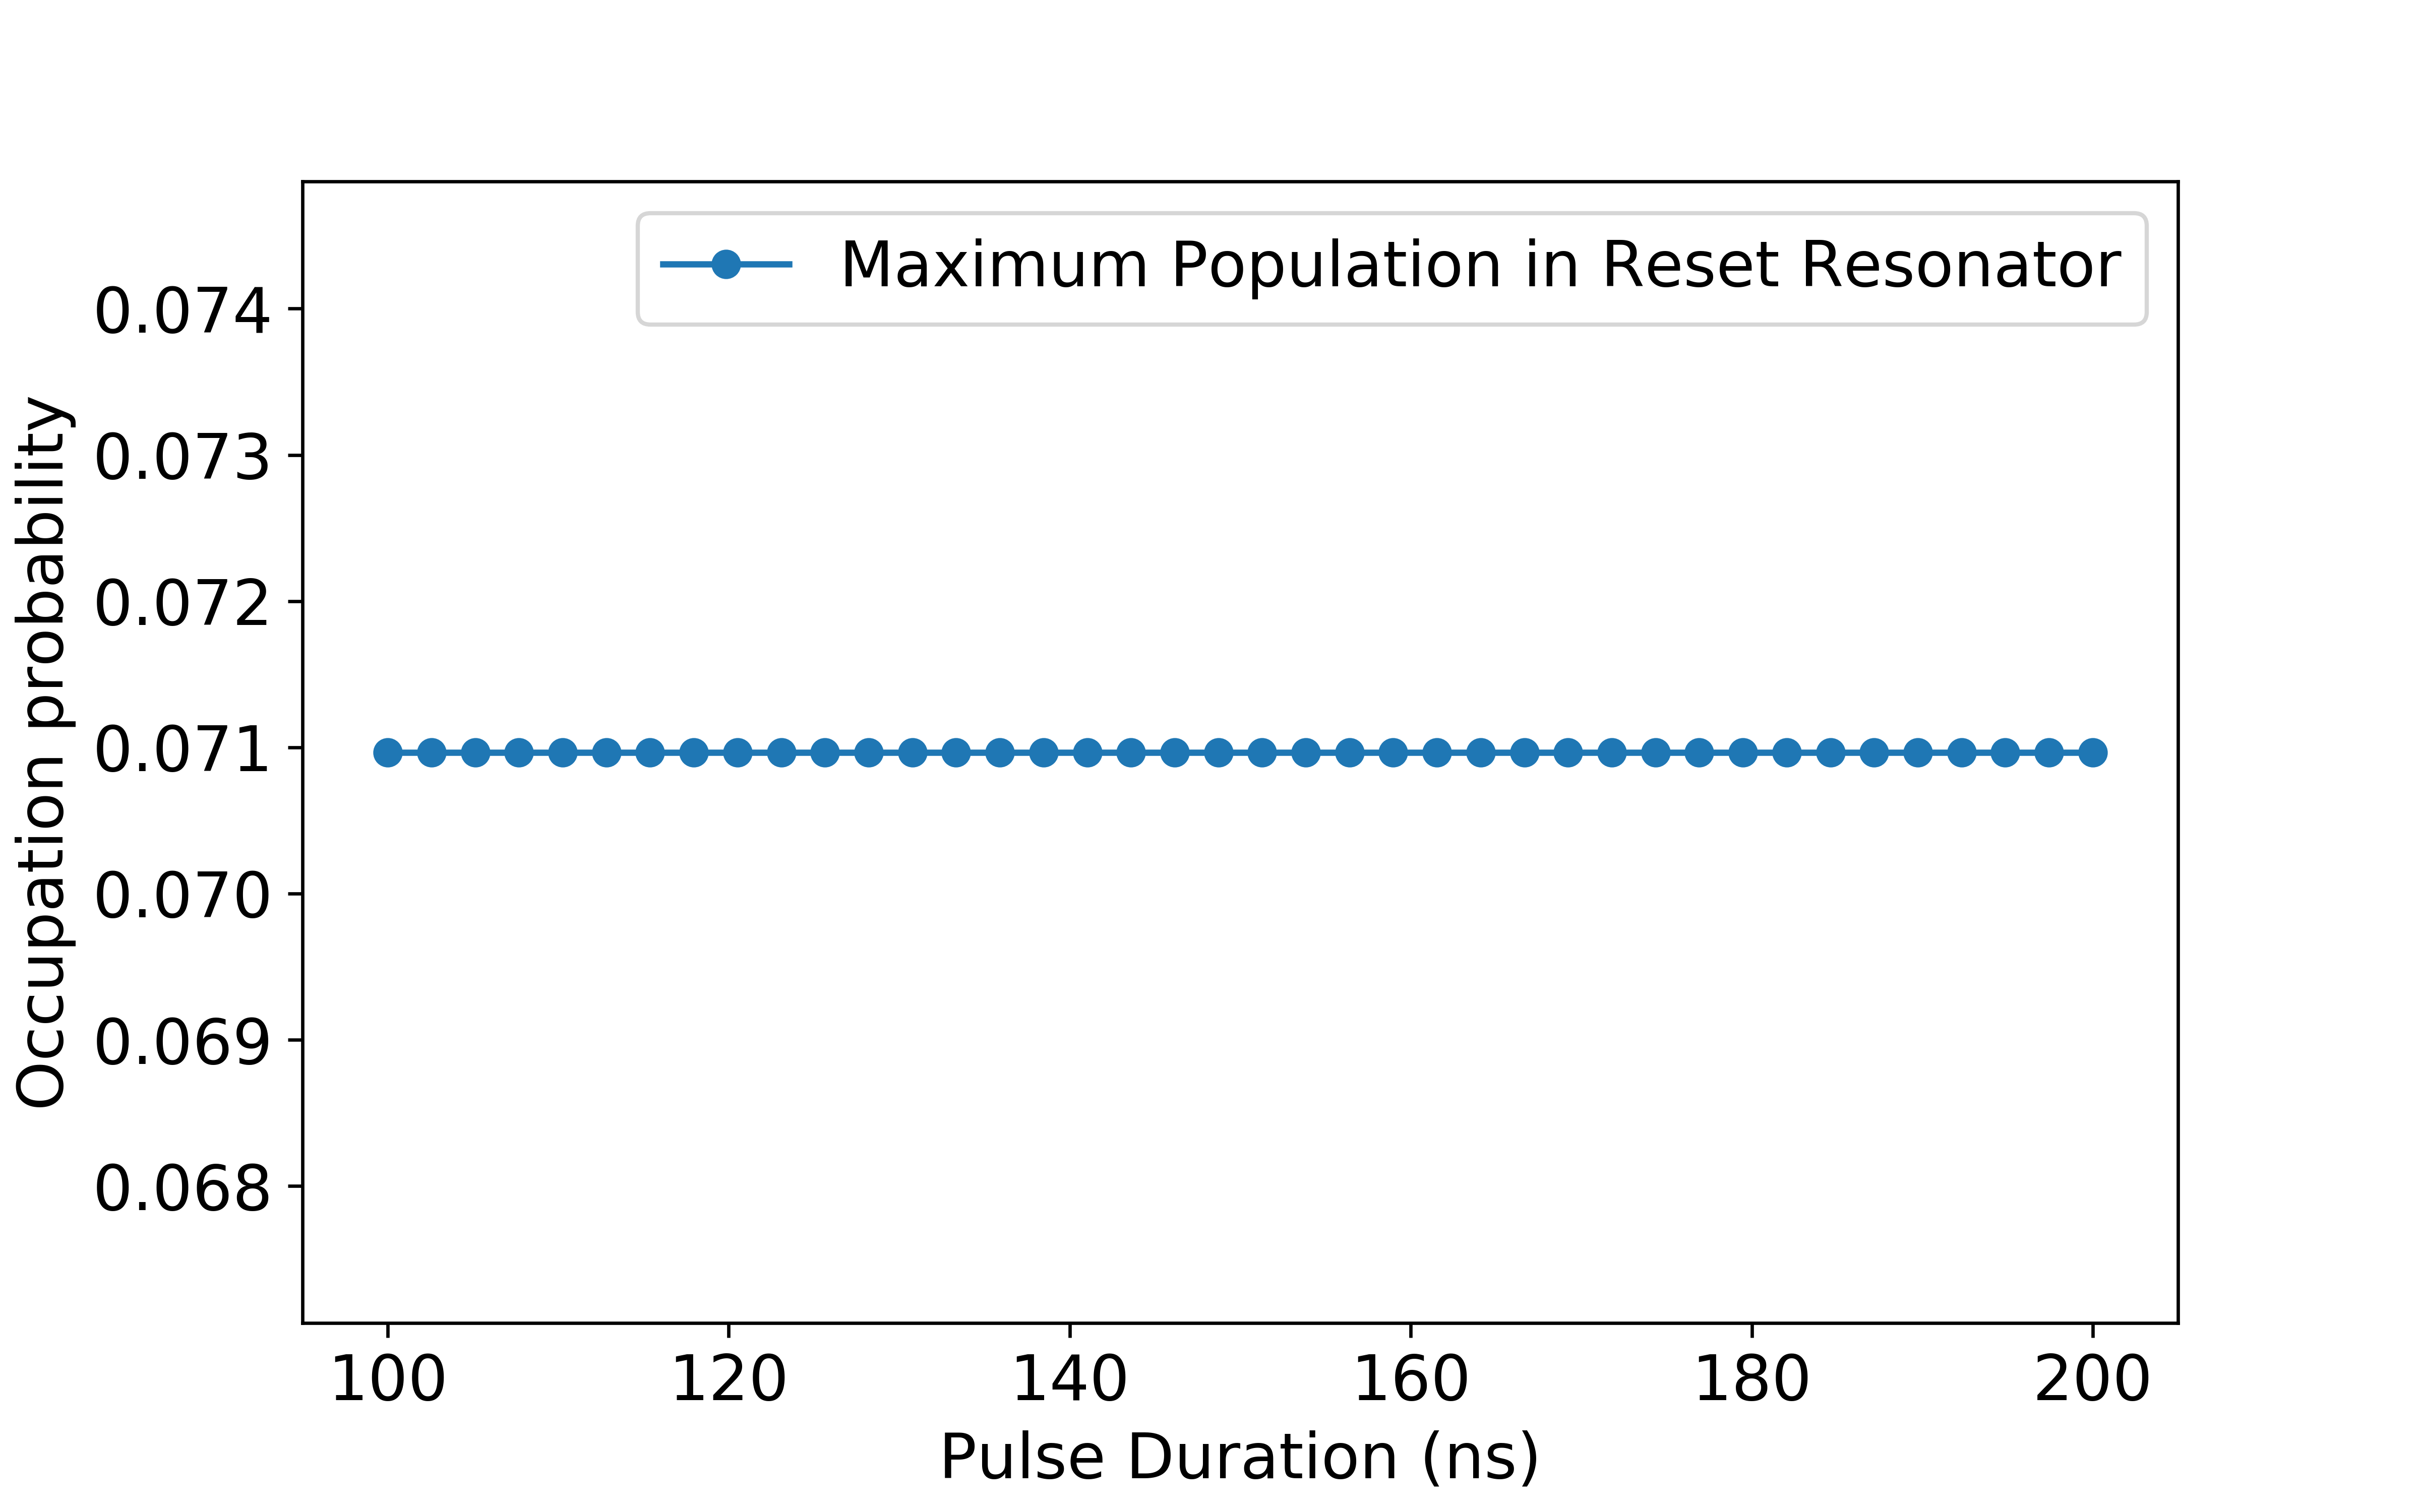
\includegraphics[width=0.6\textwidth]{pic/different_reset_schemes/reset_pop_max.png}
    \caption{The maximum value of the population of the reset resonator throughout its time evolution.}
    \label{fig:tau_sweep_reset}
\end{figure}


 While interpreting the plots in Fig. \ref{fig:tau_sweep_qubit}, the first thing that should be looked at the value of pulse duration where the population of reset resonator attains its maximum value. Since this duration signals the optimal duration of the driving pulse with specified frequency to realize a $\pi$-pulse between $\ket{f,0}$ and $\ket{g,1}$ states. In other words, higher the success of transferring the population from the qubit modes to reset modes, the faster and the more accurate reset operation. However, the population put into reset resonator is decayed too fast with compared to the Rabi timescale. Therefore, it is not possible to observe the signature of Rabi oscillation in Fig. \ref{fig:tau_sweep_qubit}. 



\begin{figure}[h!]
    \centering
    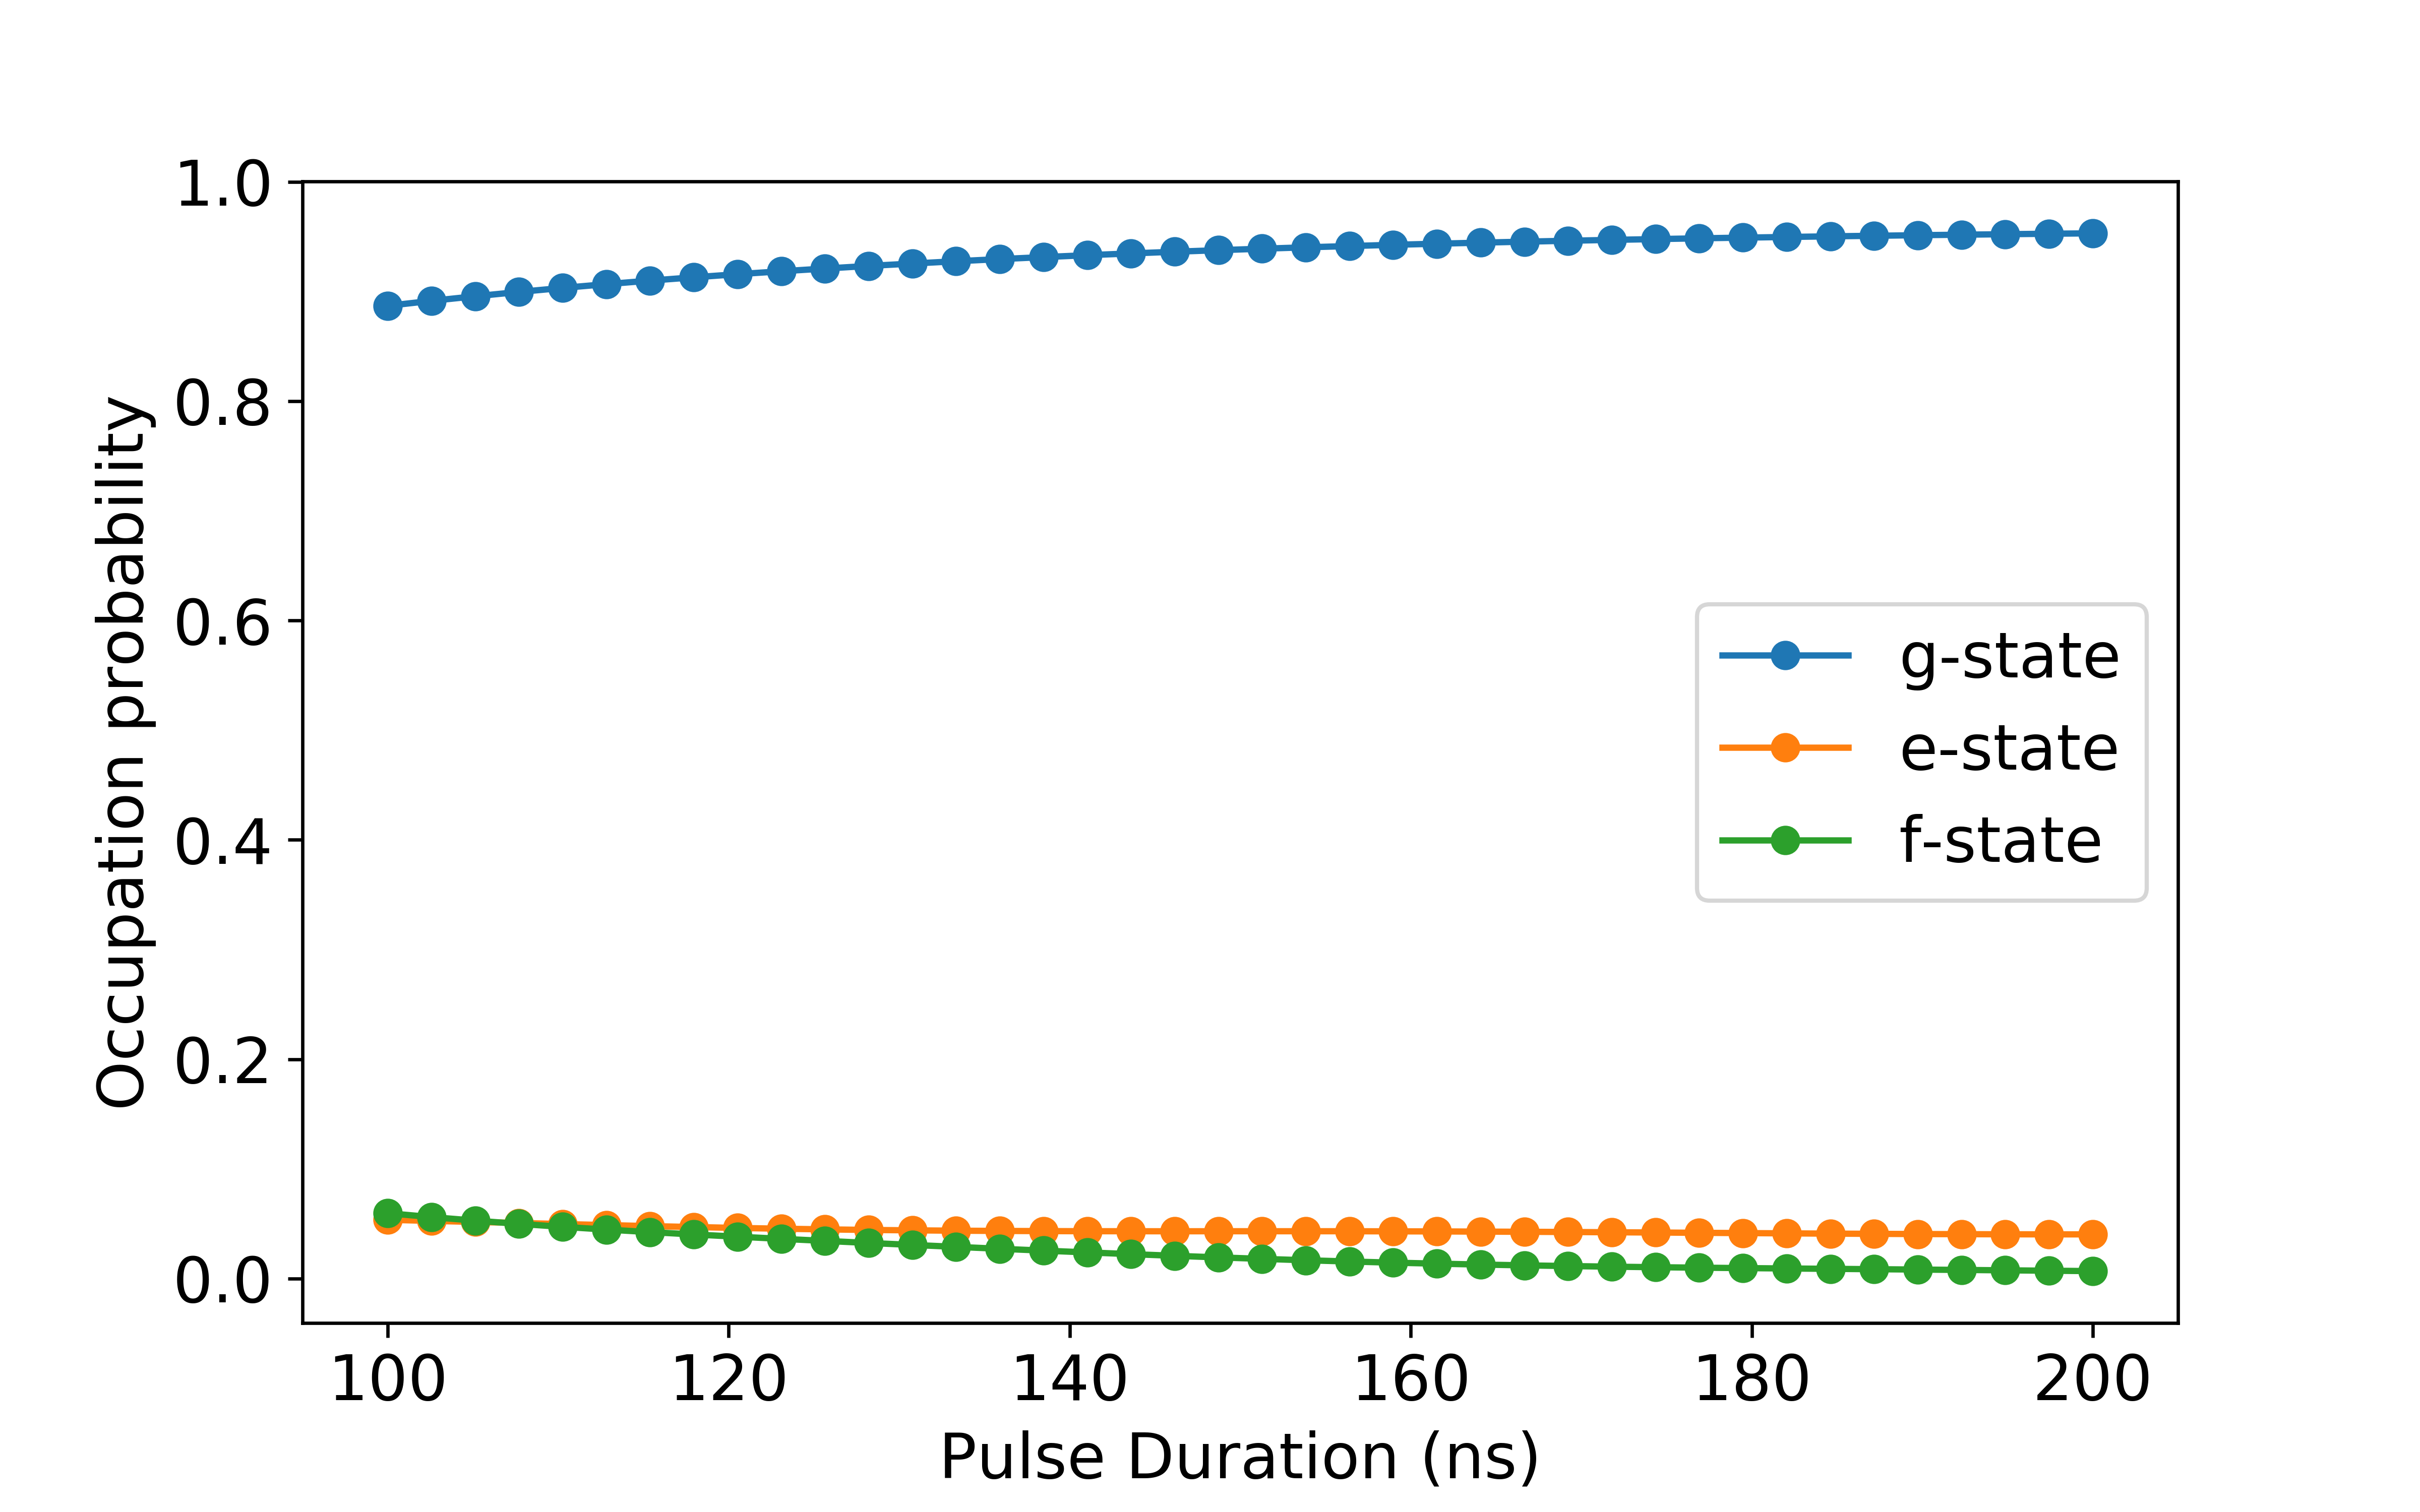
\includegraphics[width=0.6\textwidth]{pic/different_reset_schemes/gef_pops.png}
    \caption{The population of the states of the qubit.}
    \label{fig:tau_sweep_qubit_states}
\end{figure}

The prolonged application of driving pulse is forcing the population into qubit ground state, as depicted in Fig. \ref{fig:tau_sweep_qubit_states}. 




















\begin{figure}[h!]
    \centering
    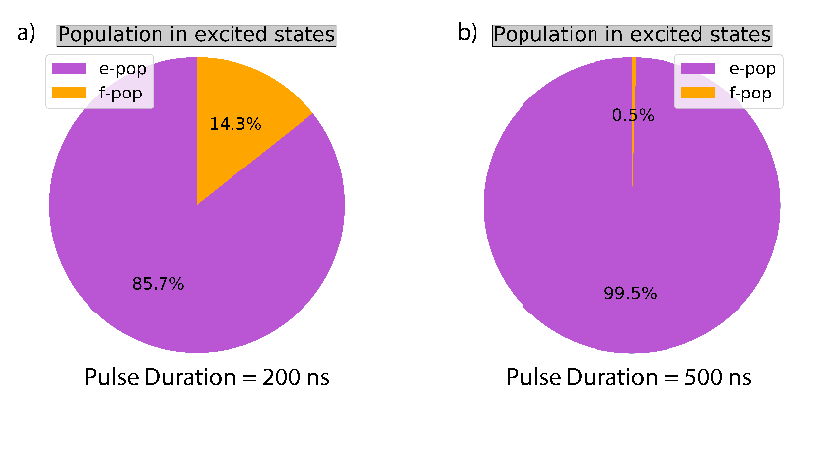
\includegraphics[width=0.6\textwidth]{pic/different_reset_schemes/dist_exc_tau_sweep.eps}
    \caption{The ratio of the population residing in $\ket{e}$ and $\ket{f}$ states for pulse duration of 200 and 500 ns. a) The overall population in excited states is The overall population in excited states is 5.6$\%$  b) The overall population in excited states is 2.5$\%$.}
    \label{fig:tau_sweep_qubit_states}
\end{figure}



























\subsection{Explanation of Functions}

\textcolor{blue}{This part could be moved in Gitlab not to overwhelm the report too much!}

\subsection{ Hamiltonian}
\textcolor{green}{This function calculates the time dependent Hamiltonian for given $\omega_{eg}$, $\omega_{read}$, $\omega_{reset}$, $\omega_{pump}$, $\alpha$, $g_1$, $g_2$, $\Omega_{d}$ (variable name as "drive rate"), $\tau$ (the length of the pulse) and $t$ (time duration of simulation), also for the simulation the  Hilbert spaces in which qubit, readout and reset mode live should be truncated. Thus, \emph{qubit trunc}, \emph{read trunc}, and \emph{reset trunc} are corresponding to the number of modes for qubit and cavities to be considered in the simulation. The Jupyter notebooks for the simulations will be made publicly available on GitHub \cite{OUR GITLAB}.
}

\subsection{Population}

In this function, the collapse operators are introduced, and QuTiP's "mesolve" function is utilized to solve the master equation corresponding to the system. This function returns the expectation value of the population of the qubit for a given time vector, $t$.







\section{Cavity-assisted quantum bath engineering}

\subsection{}
\chapter{Simulations and design of the cavity}
\section{Ansys simulation for coupled cavities}
\subsection{Frequency of the modes, field distributions, linewidths}
\subsection{Coupling strength between the two fundamental modes (the theory behind fitting [the last point in Input-Output coupling for 3D Cavity section], and the function used for fitting)}
\subsection
{Analysis of Purcell decay of qubit through each mode (it should be already in Gitlab)}
\section{Ansys and Matlab simulation for the calculation qubit's parameters}
\section{Specification sheet for the cavity}
\section{Coupling mechanism (NbTi 0.085" cables)}
\section{}
\chapter{Experimental Results}
\section{Measurement of modes in the cavity}
\section{Implementation of the branched logic}
\chapter{Branched logic applied to reset}\label{chap:branched_logic}

In this section we look at applying branched logic to reset . By branched logic we mean the ability to take decisions in real time based on experimental outcomes such as measurements. By reset, we mean going into the ground state (0) of the superconducting qubit. In particular, we will be investigating how to optimize reset using branched logic. 

Results are an improvement of two orders of magnitude in the preparation fidelity in exchange of adding a second readout pulse. A Markov chain formalism is applied to reset. 

\section{The trivial way of performing reset} \label{sec:branched_logic}

Let's have a look at the most trivial way of performing a branched logic reset. One measures the state. If 1 is measured then a $\pi$-pulse is applied to get the qubit back into the 0 state. If 0 is measured, one does nothing. The state-diagram corresponding to this is shown on figure  \ref{fig:finite_branching}. Note that the algorithm will always stop and that both branches (left, right) have different run times. We define:
\begin{itemize}
    \item $p_{0|0}$ the probability to measure 0 while the qubit being in 0,
    \item $p_{1|1}$ the probability to measure 1 while the qubit being in 1,
    \item $p_{\pi|0}$ the probability to successfully performing a $\pi$-pulse while the qubit is in 0,  
    \item $p_{\pi|1}$ the probability to successfully performing a $\pi$-pulse while the qubit is in 1.
    \item $t_\mathrm{ro}$ ($t_\pi$) the time required to readout (apply a $\pi$-pulse to) the qubit

\end{itemize}

\begin{figure}[h]
    \centering
    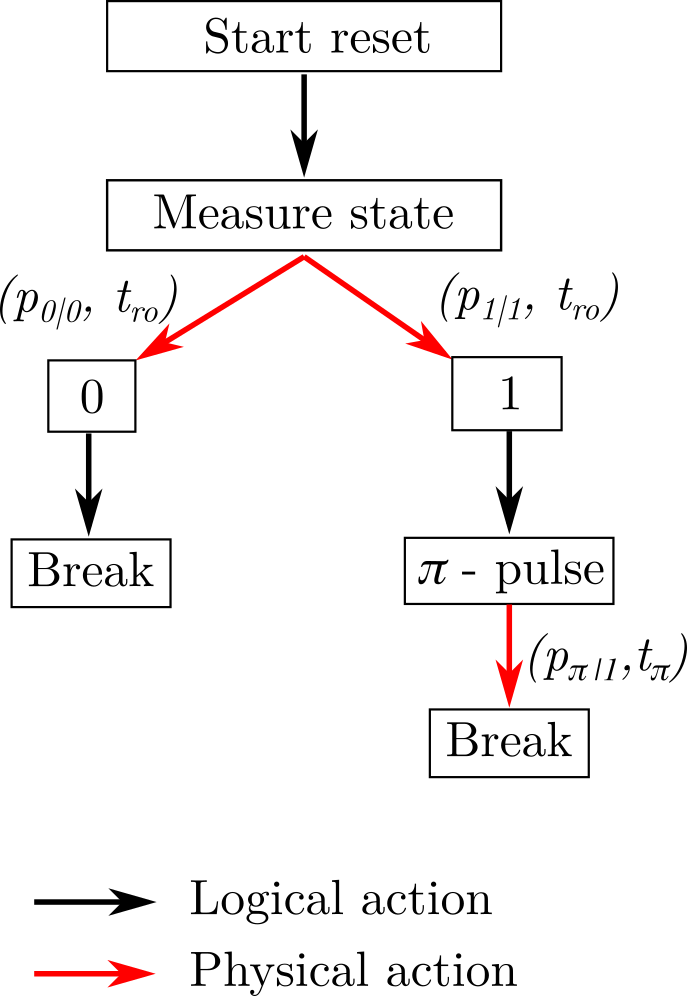
\includegraphics[width=0.5\textwidth]{pic/algorithmic_reset/finite_branching.png}
    \caption{Path-diagram for a simple reset}
    \label{fig:finite_branching}
\end{figure}

Now the question is how one can do better than the algorithm shown on figure \ref{fig:finite_branching}. For this, we want to add metrics characterizing our path-diagram. It becomes important to consider the initial state, which we assume to be $\ket{\Psi} \eqdef \alpha\ket{0} + \beta \ket{1}$.

A path is described by two properties:
\begin{itemize}
    \item \textbf{success probability}, capturing the probability $q_i$ that a path $i$ succeeds in ending in a 0 state. Note that $q_i$ is a function of initial conditions.
    \item \textbf{path time}, the time $t_i$ required to arrive at the end of the path.
\end{itemize}

A path diagram has again two properties we will be looking at: 
\begin{itemize}
    \item \textbf{total success probability}, capturing the probability $p_\textbf{success}$ the algorithm described by the diagram succeeds in resetting the qubit. 
    \item \textbf{expected termination time}, the expected time of termination $<t>$ of the algorithm.
\end{itemize}

For example, in our case one has two paths (left and right on figure \ref{fig:finite_branching}). The probabilities associated to success are given in table \ref{tab:path_finite_branching_table}.
 \begin{table}[h]
     \centering
     \begin{tabular}{c|c|c}
        Path & Success probability  & Time required \\ \hline
         Left & $q_\mathrm{left}= \abs{\alpha}^2p_{0|0}$ & $t_\mathrm{left} = t_{ro}$ \\
         Right & $q_\mathrm{right} = \abs{\beta}^2 p_{1|1}p_{\pi|1}$ & $t_\mathrm{right} = t_{ro} + t_\pi$
     \end{tabular}
     \caption{Table summarizing the success probabilities of paths shown on figure \ref{fig:finite_branching}. }
     \label{tab:path_finite_branching_table}
 \end{table}

Assuming for example $p_{0|0} = p_{1|1} = p_{\pi|} = p_{\pi|1} = 99\%, \abs{\alpha}^2  = 0.5$ one finds that $p_\text{success} = 98.505 \%$ and that $<t> =  t_{ro} + 0.495 t_\pi$.



\section{Branched logic approach to reset}
The algorithm presented in section \ref{sec:branched_logic} will always terminate after one run. However, in order to improve reset fidelity, one can decide to measure the qubit and applying a $\pi$-pulse \textit{while} seeing a 1 state. Once a ground state is measured, the algorithm stops. A path-diagram corresponding to this algorithm is given on figure \ref{fig:infinite_branching}.

\begin{figure}[h]
    \centering
    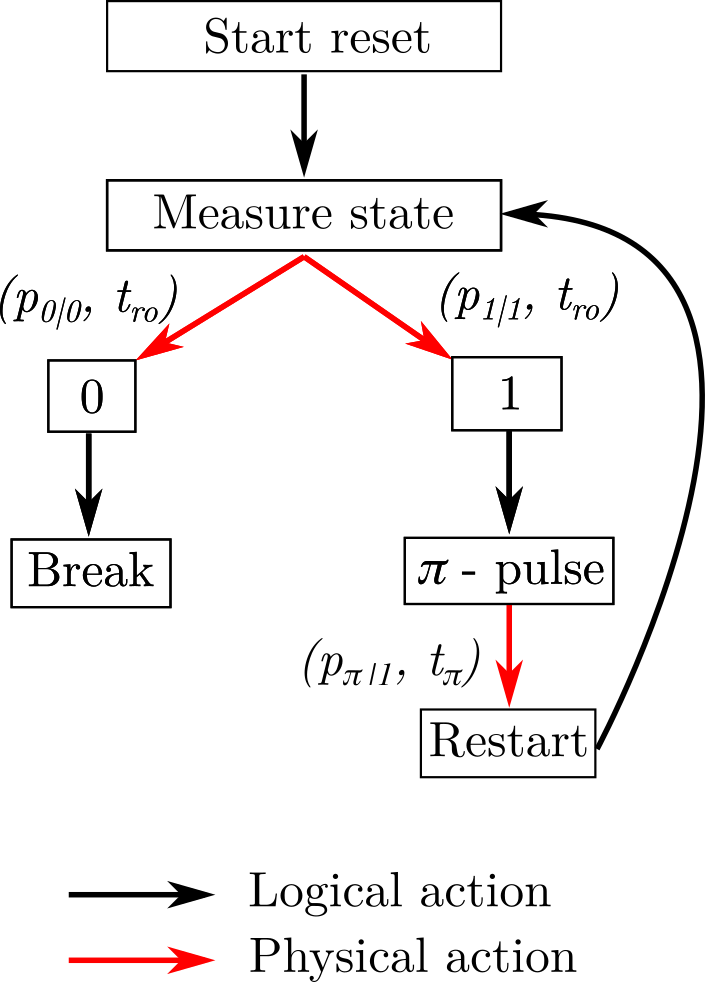
\includegraphics[width=0.5\textwidth]{pic/algorithmic_reset/infinite_branching.png}
    \caption{Ansatz on maximising state preparation fidelity}
    \label{fig:infinite_branching}
\end{figure}

Computing the probabilities and times associated to each path yields the results shown on table \ref{tab:path_infinite_branching_table}. It becomes obvious that manually computing paths and their probabilities is not possible anymore. In order to solve this, we introduce the Transition Matrix formalism.

 \begin{table}[H]
     \begin{tabular}{c|c|c|c}
       Path index $i$ & Path & Success probability $p_i$ & Time required \\ \hline
        0 & Left & $\abs{\alpha}^2 p_{0|0}$ & $t_{ro}$ \\
        1 &  Right, left & $\abs{\beta}^2p_{1|1}p_{\pi|1}p_{0|0}$ & $2t_{ro} + t_\pi$ \\
        2 &  Right, right, left & $\abs{\beta}^2 p_{1|1}^2 (1-p_{\pi|1}) p_{\pi|1} p_{0|0} + \abs{\alpha}^2 p_{1|0} p_{\pi|1} p_{1|1} p_{\pi|1} p_{0|0} $ & $3t_{ro} + 2t_\pi$ \\
         ... & ... & ... & ... \\
        n & (Right)$^n$, left & $p_{1|1}^np_{\pi|1}^np_{0|0} + \mathcal{O}(\epsilon)$ & $(n+1)t_{ro} + nt_\pi$ \\
        ... & ... & ... & ...
     \end{tabular}
     \caption{Table summarizing the success probabilities of paths shown on figure \ref{fig:infinite_branching}. $\epsilon$ is of the order of the probability that an operation goes wrong}
     \label{tab:path_infinite_branching_table}
 \end{table}
 
 \subsection{Transition matrix formalism}

% In fact what we are facing here is a decision problem.

We will introduce a formalism allowing us to compute success probabilities. 

%We have access to incomplete information about our system, and take actions accordingly. 
%% Insert picture knowledge => action => update knowledge. 

Our state diagram can be seen as a set of states. A state is defined by the knowledge of the qubit we have (ie. the measurement) and the actual state of the qubit. A list of states is given on table \ref{tab:states_branching1}.
 
 \begin{table}[h]
     \centering
     \begin{tabular}{c|c|c|c}
        State tag $s_i$ & State name & Description & Next action \\ \hline 
        $s_1$ & $0|0$  & 0 measured, qubit is in state 0 & \textbf{Break}\\ 
        $s_2$ & $0|1$  & 0 measured, qubit is in state 1 & \textbf{Break}\\ 
        $s_3$ & $1|0$  & 1 measured, qubit is in state 0 & Apply $\pi$-pulse, measure again\\ 
        $s_4$ & $1|1$  & 1 measured, qubit is in state 1 & Apply $\pi$-pulse, measure again
     \end{tabular}
     \caption{List of states of the path-diagram and of the actions taken.}
     \label{tab:states_branching1}
 \end{table}

After each round of algorithm one goes from one state to another with a certain probability. This is a Markov Chain setting. 

Note that the desired state is $s_1$. Once in $s_1$, we don't leave it anymore, it's an irreversible action. Similarly, reaching $s_2$ also is irreversible with the difference that being in $s_2$ means having failed the reset. To each path from $s_i$ to $s_j$ we can associate a transition probability $p_{j\leftarrow i} = (T)_{ji}$, giving us a Markov transition matrix $T$. In our case we have 
\begin{equation}
    T = \left(
\begin{array}{cccc}
 1 & 0 & {p_{0|0}} (1-{p_{\pi|0}}) & {p_{0|0}} {p_{\pi|1}} \\
 0 & 1 & (1-{p_{1|1}}) {p_{\pi|0}} & (1-{p_{1|1}}) (1-{p_{\pi|1}}) \\
 0 & 0 & (1-{p_{0|0}}) (1-{p_{\pi|0}}) & (1-{p_{0|0}}) {p_{\pi|1}} \\
 0 & 0 & {p_{1|1}} p_{\pi|0} & {p_{1|1}} (1-{p_{\pi|1}}) \\
\end{array}
\right)
\end{equation}

The matrix describes the evolution of the system. Defining a state vector $\Vec{P_k} = \bmat{P_{s_1}, P_{s_2}, P_{s_3}, P_{s_4}}^\top$ containing the probabilities $P_{s_i}$ of being in state $i$ after iteration $k$ we can investigate the time-evolution. Our initial state is given by 

\begin{equation}
    \Vec{P_0} = \bmat{\abs{\alpha}^2 p_{0|0}\\(\abs{\beta}^2) (1 - p_{1|1})\\\abs{\alpha}^2(1- p_{0|0})\\\abs{\beta}^2 p_{1|1}}. \label{eq:Pk}
\end{equation}

and the state after $k$ iterations is given by

\begin{equation}
   \Vec{P_k} = T^k \Vec{P_0}.
\end{equation}

\subsubsection{Computing the asymptotic evolution of the state-vector}

One can analytically compute the convergence of the scheme. Let $\left\{\vec e_i\right\}_{i\in \mathrm{states}}$ be the eigenvectors of $T$, and let $\left\{\lambda_i\right\}_{i\in \mathrm{states}}$ be the corresponding eigenvalues. Let $\left\{\gamma_i\right\}_{i\in \mathrm{states}}$ be such that 
\begin{equation}
    \vec P_0 = \sum_{i\in \mathrm{states}} \gamma_i \vec e_i.
\end{equation}

Then one has that 

\begin{equation}
    \vec P_k = T^k \vec P_0 =  \sum_{i\in \mathrm{states}} \gamma_i \lambda_i^k  \vec e_i.
\end{equation}

The eigenvalues of $T$ are (first analytically, then for $p_{0|0} = p_{1|1} = p_{\pi|} = p_{\pi|1} = 0.99$): 
\begin{eqnarray}
\lambda_1 = 1 \\
\lambda_2 = 1
\end{eqnarray}
\begin{equation}
\begin{split}
\lambda_3 = \frac{\sqrt{(p_{0|0} (-p_{\pi|0})+p_{0|0}+p_{1|1} (p_{\pi|1}-1)+p_{\pi|0}-1)^2-4 (p_{0|0}-1) p_{1|1} (p_{\pi|0}+p_{\pi|1}-1)}}{2} \\
+\frac{p_{0|0} (p_{\pi|0}-1)+p_{1|1} (-p_{\pi|1})+p_{1|1}-p_{\pi|0}+1}{2} \approx 0.1
\end{split}
\end{equation}

\begin{equation}
\begin{split}
\lambda_4 = \frac{-\sqrt{(p_{0|0} (-p_{\pi|0})+p_{0|0}+p_{1|1} (p_{\pi|1}-1)+p_{\pi|0}-1)^2-4 (p_{0|0}-1) p_{1|1} (p_{\pi|0}+p_{\pi|1}-1)}}{2} \\
+\frac{p_{0|0} (p_{\pi|0}-1)+p_{1|1} (-p_{\pi|1})+p_{1|1}-p_{\pi|0}+1}{2} \approx -0.09
\end{split}
\end{equation}

This shows that our scheme will exponentially converge into the $\mathrm{span}(\vec e_1, \vec e_2)$ subspace: repeatedly applying $T$ will exponentially suppress the components in $\mathrm{span}(\vec e_3, \vec e_4)$ as $\abs{\lambda_3}, \abs{\lambda_4} < 1$. We have that $\vec e_1 = \bmat{1, 0, 0, 0}^\top$ and $\vec e_2 = \bmat{0, 1, 0, 0}^\top$, corresponding to the state of the algorithm having terminated. This is reassuring as this means that our algorithm will terminate in a finite time with probability 1. 

The other eigenvectors can be found in the file \textit{path\_analysis.nb} (their analytical expression is - well - long). They are a linear combination of all components. %% add here exactly where to find it for future use

It is worth to note that the sum of components of $\vec e_1, \vec e_2$ equals 1, whereas for $\vec e_3, \vec e_4$ it equals 0. %% More discussion? 


We analytically find $\gamma_1, \gamma_2$ as they allow us to compute the asymptotic state. We find: 

\begin{equation}
    \lim_{k \to \infty}\Vec{P_k} = \lim_{k \to \infty} \sum_{i=1}^4 \gamma_i \vec e_i \lambda_i ^k = \bmat{\gamma_1 \\ \gamma_2\\0 \\ 0}.
\end{equation}

This not only gives us an asymptotic evolution but also a measure of how quickly we converge: the runtime of the algorithm is in $\mathcal{O} \left((\max_{i \in {3,4}}\abs{\lambda_i})^k\right)$. \textit{(not sure if one can say that this way - what I mean is that the probability of not having reset after k rounds decreases exponentially, the expected runtime can be easily computed as can be found below}

Furthermore, one can exactly compute probability of success and of failure: $\gamma_2$ is the probability that our scheme fails, $\gamma_1$ is the probability to succeed in the reset. Computing $\gamma_1$ and $\gamma_2$ for $\vec P_0$ as given in equation \ref{eq:Pk} one obtains: 

\begin{equation}
    \begin{split}
        \gamma_1 = \frac{p_{0|0} \left(\alpha ^2+p_{1|1} \left(p_{\pi|1}-\alpha ^2\right)\right)}{p_{0|0} (1-p_{1|1}) (1-p_{\pi|0})+p_{0|0} p_{1|1} p_{\pi|1}+ p_{\pi|0}(1-p_{1|1})},
    \end{split}
\end{equation}

\begin{equation}
    \begin{split}
       \gamma_2 = \frac{(1-p_{1|1}) \left(p_{0|0} \left(1-\alpha ^2-p_{\pi|0}\right)+p_{\pi|0}\right)}{p_{0|0} (1-p_{1|1}) (1-p_{\pi|0})+p_{0|0} p_{1|1} p_{\pi|1} + p_{\pi|0}(1-p_{1|1})}
    \end{split}
\end{equation}

with $\gamma_1 + \gamma_2 = 1$. This gives us an exact prediction of what the success probability of our reset scheme are, the probability of success being given by $\gamma_1$ and the probability of failure by $\gamma_2$.

Using the "toy values" $p_{0|0} = p_{1|1} = p_{\pi|} = p_{\pi|1} = 0.99$, one can compare success probabilities as a function of $\abs{\alpha}^2$. One finds:
\begin{equation}
    p_\text{success} = 98.99 \% + 0.010099 \cdot \abs{\alpha}^2 \overset{\abs{\alpha}^2 = \frac{1}{2}}{=} 99.48 \%
\end{equation}



Note that there is a 1\% increase compared to the previous scheme. 

The main error source could to be investigated thoroughly, but intuitively one can see that the main error contribution happens at the first step when wrongfully measuring a 0 state. The success probability can be further enhanced as will be discussed in section \ref{sec:double_readout}.  

\subsubsection{Computing termination time}

Using Mathematica, it is straightforward to compute $\Vec{P_k}$ for a set of starting values. An example of an evolution is given on figure \ref{fig:p_k}.

\begin{figure}[h]
    \centering
    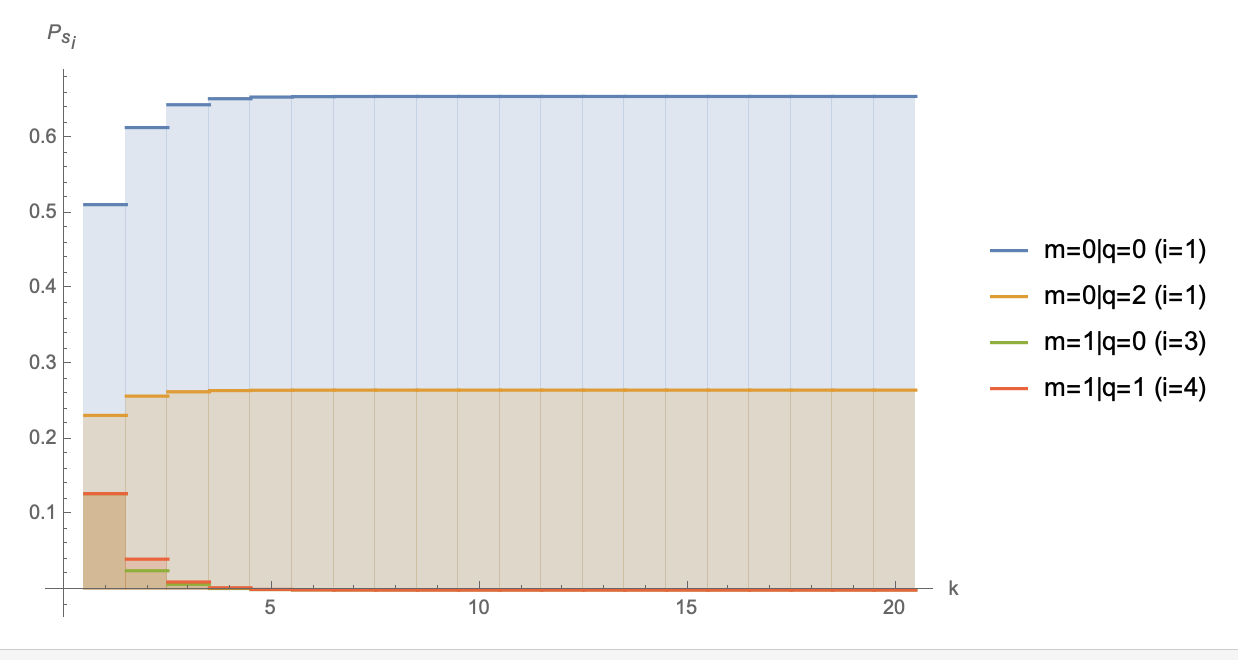
\includegraphics[width=0.6\textwidth]{state_prop_evol_i=4.png}
    \caption{\textbf{(to be
    changed: this figure was generated with a small bug in the code. Starting values should be adjusted for a nicer picture)}. Note that there is a residual population in the $s_2$ state, which means our reset is not working perfectly. }
    \label{fig:p_k}
\end{figure}

This allows computing the expected time of reset $<t>$: 

\begin{equation}
\begin{split}
    < t > = \sum_{k = 0 }^\infty \underbrace{\left[P_{s_1,k+1} + P_{s_2,k+1} - (P_{s_1,k} + P_{s_2,k})\right]}_{\text{Probability of terminating after } k+1 \text{ steps}}\underbrace{(t_{ro} + t_\pi)(k+1)}_{\text{time process took}} - \underbrace{t_{\pi}}_{\text{no pulse once 0 measured}}\\ 
\end{split}
\end{equation}

This can be further simplified to 

\begin{equation}
\begin{split}
    < t > = \sum_{k = 0 }^\infty \underbrace{\left[\gamma_1 + \gamma_2 - \gamma_3\lambda_3^k((\vec{e_3})_1 + (\vec{e_3})_2) - \gamma_4\lambda_4^k((\vec{e_4})_1 + (\vec{e_4})_2) \right]}_{\text{Probability of terminating after } k+1 \text{ steps}}\underbrace{(t_{ro} + t_\pi)(k+1)}_{\text{time process took}} \\
    - \underbrace{t_{\pi}}_{\text{no pulse once 0 measured}}\\ 
\end{split}
\end{equation}

Which are all values we have computed previously. Unfortunately, getting the analytical solution is not very instructive, so plugging some numbers into the equations helps us seeing clearer. Assuming again $p_{0|0} = p_{1|1} = p_{\pi|} = p_{\pi|1} = 0.99, \abs{\alpha}^2  = 0.5$, we have that: 

\begin{equation}
    <t> = t_{ro} + (0.9947 - \abs{\alpha}^2 0.9548) (t_{ro} + t_\pi) \overset{\abs{\alpha}^2 = \frac{1}{2}}{=} t_{ro} + 0.5173(t_{ro} + t_\pi)
\end{equation}

where one sees that on average the time difference between this and the previous scheme is approximately $t_{ro}$. So for the price of one more readout one gets around 1\% improvement for our "toy" values.  





\section{Improving the reset probability} \label{sec:double_readout}

The main source of error in the previously proposed scheme is when wrongly measuring a 0. To avoid this happening one can decide reading out a second time to ensure that we start with a correct state.

A state diagram is shown on figure \ref{fig:double_infinite_branching}. 

\begin{figure}[h]
    \centering
    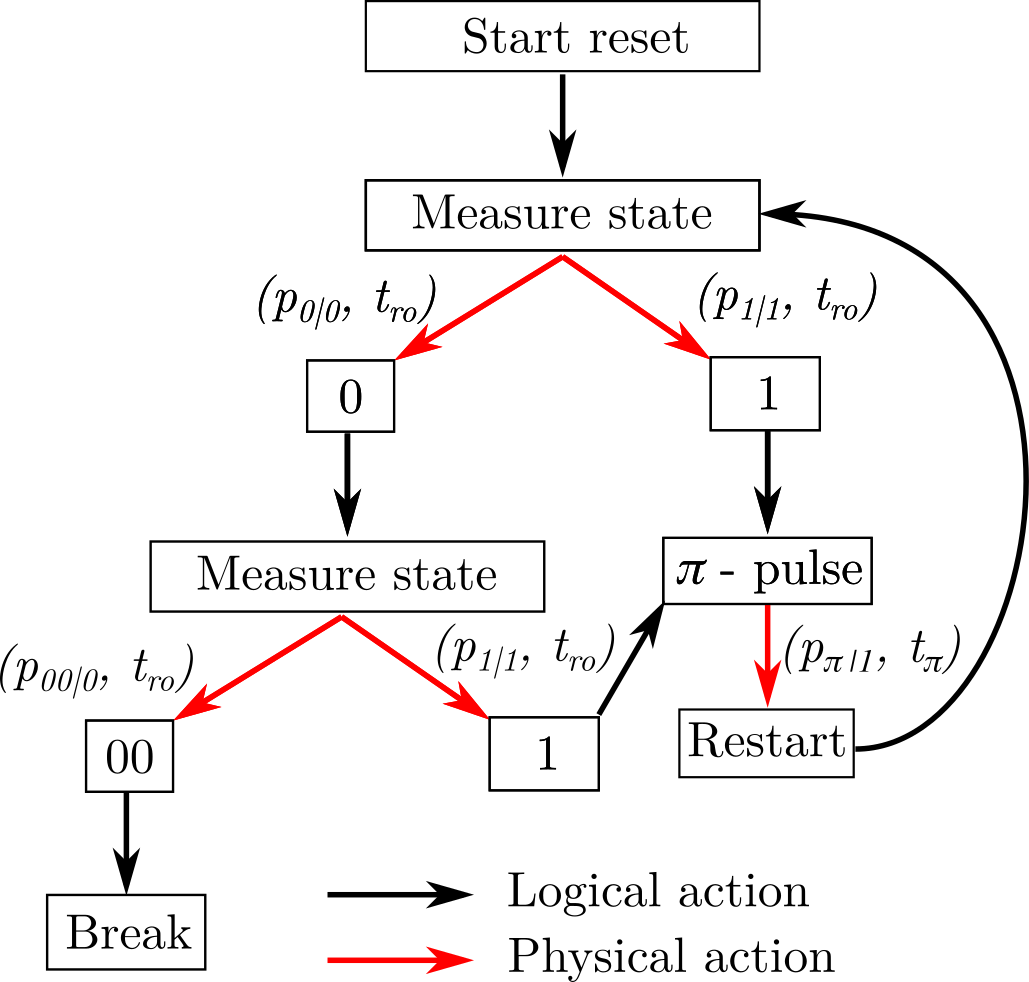
\includegraphics[width=0.5\textwidth]{pic/algorithmic_reset/double_infinite_branching.png}
    \caption{Caption}
    \label{fig:double_infinite_branching}
\end{figure}

A list of states is given on table \ref{tab:states_branching2}

 
 \begin{table}[h]
     \centering
     \begin{tabular}{c|c|c|c}
        State tag $s_i$ & State name & Description & Next action \\ \hline 
        $s_1$ & $0|0$  & 0 measured, qubit is in state 0 & Measure again \\ 
        $s_2$ & $0|1$  & 0 measured, qubit is in state 1 & Measure again \\ 
        $s_3$ & $1|0$  & 1 measured, qubit is in state 0 & Apply $\pi$-pulse, measure again \\ 
        $s_4$ & $1|1$  & 1 measured, qubit is in state 1 & Apply $\pi$-pulse, measure again \\
        $s_5$ & $00|0$  & 0 measured twice, qubit is in state 0 & \textbf{Break} (successful) \\
        $s_6$ & $00|1$  & 0 measured twice, qubit is in state 1 & \textbf{Break} (unsuccessful) \\
        
     \end{tabular}
     \caption{List of states of the path-diagram for improved reset fidelty}
     \label{tab:states_branching2}
 \end{table}


Applying the same treatment as before, but now in a 6-dimensional state-space one has: 

\begin{equation}
    \Vec{P_0} = \bmat{\abs{\alpha}^2 p_{0|0}\\(\abs{\beta}^2) (1 - p_{1|1})\\\abs{\alpha}^2(1- p_{0|0})\\\abs{\beta}^2 p_{1|1} \\ 0 \\ 0}. \label{eq:Pk6}
\end{equation}
%% Markov transition Matrix

\begin{equation}
    T = \bmat{0 & 0 & p_{0|0}(1-p_{\pi|0}) & p_{0|0} p_{\pi|1} & 0 & 0 \\ 
    0 & 0 & (1-p_{1|1})p_{\pi|0} & (1-p_{1|1})(1-p_{\pi|1}) & 0 & 0 \\ 
    (1-p_{0|0}) & 0 & (1-p_{0|0})(1-p_{\pi|0}) & (1-p_{0|0})p_{\pi|1} & 0 & 0 \\
    0 & p_{1|1} & p_{1|1}p_{\pi|0} & p_{1|1}(1-p_{\pi|1}) & 0 & 0\\ 
    p_{0|0} & 0 & 0 & 0 & 1 & 0 \\
    0 & (1-p_{1|1}) & 0 & 0 & 0 & 1}
\end{equation}

$T$ again has the same properties as before, namely that we have two unity eigenvalues corresponding to the final states $s_5$ and $s_6$. The eigenvalues corresponding to the other eigenstates are $|\cdot| < 1$. One can, using the same method as previously, compute the probabilities of success. All files describing the calculations can be found in the files \textit{path\_analysis.nb} and \textit{path\_analysis.m}. Note that computing eigenvalues and eigenvectors analytically for the $6\times6$ matrix $T$ is not realistic anymore, therefore it was chosen to simply leave $t_{ro}$ and $t_{\pi}$ as symbolic variables when computing $<t>$. Note also that the formula for $<t>$ slightly changes: 

\begin{equation}
\begin{split}
    < t > = \sum_{k = 0 }^\infty \underbrace{\left[P_{s_5,k+1} + P_{s_6,k+1} - (P_{s_5,k} + P_{s_6,k})\right]}_{\text{Probability of terminating after } k+1 \text{ steps}}\underbrace{(t_{ro} + t_\pi)(k+1)}_{\text{time process took}} \\ + \underbrace{t_{ro}}_{\text{initialization time}} - \underbrace{t_{\pi}}_{\text{no pulse once 0 measured}}\\ 
\end{split}
\end{equation}

Results are the following, again for our toy model with probabilities $p_{0|0} = p_{1|1} = p_{\pi|} = p_{\pi|1} = 0.99$. 

\begin{eqnarray}
p_\text{success} = 99.99\% + 1.01\e{-4} \abs{\alpha}^2  \overset{\abs{\alpha}^2 = \frac{1}{2}}{=} 99.995 \% \\
<t> = (2.0709 - 1.02 \abs{\alpha}^2)(t_\pi + t_{ro}) + t_{ro} \overset{\abs{\alpha}^2 = \frac{1}{2}}{=} 1.5609(t_\pi + t_{ro}) + t_{ro}
\end{eqnarray}

Here it becomes clear that by paying a small time tribute one can significantly improve the reset success probability.

\section{Optimization choices}

A reset protocol is usually followed by an experiment, which will last a certain amount of time $t_\mathrm{exp}$.
Two optimisation routes can be taken:
\begin{enumerate}
    \item maximize the number of experiments starting with a successful reset, which means taking the state-diagram maximizing
    \begin{equation}
        \sum_{i \in \mathrm{paths}} q_i(t_i + t_\mathrm{exp}), \label{eq:pathtime-optimizer}
    \end{equation}
    \item minimize the number of experiments starting with a wrongly reset state, which means taking the diagram maximizing
    \begin{equation}
        \sum_{i \in \mathrm{paths}}  q_i,
    \end{equation}
\end{enumerate} 

where $q_i$ is the probability to take path $i$ successfully (ie. that one takes path $i$ and that you end up in the ground state) and $t_i$ the length of the path. 

Option 1 means maximizing the number of successful experiments while paying the price of starting sometimes with a wrong state. This option could be interesting if one can post-select on wrongly prepared states or if one can live with errors. If one decides to run an algorithm where the correctness of the answer is easily checked (e.g. factorisation of prime numbers) this option should be favoured.

Option 2 means trying everything you can do to be absolutely sure to start in the right state. This is the option maximizing experiment fidelity, to be chosen whenever one cannot post-select on the outcome of an experiment. 

Note that in the limit of $t_i \ll t_\mathrm{exp} \forall i \in \mathrm{paths}$, option 1 becomes equivalent to option 2. Also, this reasoning generalizes to any case where one has a trade-off between speed and accuracy. 

Finally, it would be interesting to compute numbers for equation \ref{eq:pathtime-optimizer}. One could for example numerically compute: 

\begin{equation}
\begin{split}
    < t > = \sum_{k = 0 }^\infty \underbrace{\left[P_{s_5,k+1} - P_{s_5,k})\right]}_{\text{Probability of success after } k+1 \text{ steps}}\cdot \underbrace{(t_{ro} + t_\pi)(k+1)}_{\text{time process took}} \\ + \underbrace{t_{ro}}_{\text{initialization time}} - \underbrace{t_{\pi}}_{\text{no pulse once 0 measured}}\\ 
\end{split}
\end{equation}

this has not been further investigated but could provide useful for short experiments where the correctness of the outcome can be assessed. 
\chapter{Conclusion and outlook}
\section{Implementing branched logic into PyCQED}
\printbibliography

\end{document}
